\documentclass[12pt,a4paper]{report}

% Required Packages
\usepackage[utf8]{inputenc}
\usepackage[english]{babel}
\usepackage{geometry}
\usepackage{graphicx}
\usepackage{amsmath}
\usepackage{amssymb}
\usepackage{setspace}
\usepackage{titlesec}
\usepackage{fancyhdr}
\usepackage{hyperref}
\usepackage{cite}
\usepackage{caption}
\usepackage{subcaption}
\usepackage{float}
\usepackage{listings}
\usepackage{xcolor}
\usepackage{tocloft}
\usepackage{parskip}
\usepackage{booktabs}
\usepackage{multirow}
\usepackage{array}
\usepackage{longtable}

% Page Geometry
\geometry{left=1.5in, right=1in, top=1in, bottom=1in}

% Line Spacing
\onehalfspacing

% Header and Footer
\pagestyle{fancy}
\fancyhf{}
\fancyhead[R]{\thepage}
\renewcommand{\headrulewidth}{0.4pt}

% Hyperref Settings
\hypersetup{
    colorlinks=true,
    linkcolor=black,
    citecolor=blue,
    urlcolor=blue,
    pdftitle={Multimodal Relationship Extraction in Twitter Data Using Deep Learning},
    pdfauthor={Your Name}
}

% Title Formatting
\titleformat{\chapter}[display]
{\normalfont\huge\bfseries}{\chaptertitlename\ \thechapter}{20pt}{\Huge}
\titlespacing*{\chapter}{0pt}{-20pt}{40pt}

% Code Listing Settings
\lstset{
    basicstyle=\ttfamily\small,
    breaklines=true,
    frame=single,
    numbers=left,
    numberstyle=\tiny,
    keywordstyle=\color{blue},
    commentstyle=\color{green},
    stringstyle=\color{red}
}

% Graphics path
\graphicspath{{./}}

\begin{document}

% ==========================================
% FRONT PAGE
% ==========================================
\begin{titlepage}
    \centering
    \vspace*{1cm}
    
    {\LARGE\textbf{MULTIMODAL RELATIONSHIP EXTRACTION IN TWITTER DATA USING DEEP LEARNING}}\\[1.5cm]
    
    {\Large Mid-Term Thesis Report}\\[0.5cm]
    {\large Submitted in Partial Fulfillment of the Requirements}\\
    {\large for the Degree of}\\[0.5cm]
    {\Large\textbf{Master of Science in Computer Science}}\\[2cm]
    
    {\large \textbf{Submitted by:}}\\[0.3cm]
    {\Large Your Name}\\
    {\large Roll No: XXXXXXX}\\[2cm]
    
    {\large \textbf{Under the Supervision of:}}\\[0.3cm]
    {\Large Dr. Supervisor Name}\\
    {\large Professor, Department of Computer Science}\\[2cm]
    
    \vfill
    
    {\large\textbf{DEPARTMENT OF COMPUTER SCIENCE}}\\
    {\large\textbf{YOUR UNIVERSITY NAME}}\\
    {\large\textbf{City, Country}}\\[0.5cm]
    {\large\textbf{\today}}
    
\end{titlepage}

% ==========================================
% CERTIFICATE / DECLARATION (Optional)
% ==========================================
\chapter*{Certificate}
\thispagestyle{empty}
This is to certify that the work entitled \textbf{"Multimodal Relationship Extraction in Twitter Data Using Deep Learning"} is an original work carried out by \textbf{Your Name}, under my supervision and guidance for the partial fulfillment of the requirements for the degree of Master of Science in Computer Science at Your University Name.

\vspace{2cm}

\noindent
\textbf{Dr. Supervisor Name}\\
Professor\\
Department of Computer Science\\
Your University Name\\
Date: \underline{\hspace{3cm}}

\cleardoublepage

% ==========================================
% ABSTRACT
% ==========================================
\chapter*{Abstract}
\addcontentsline{toc}{chapter}{Abstract}
\thispagestyle{empty}

The exponential growth of social media platforms has generated massive volumes of multimodal content combining textual narratives with visual imagery. Twitter, as one of the most influential microblogging platforms, presents unique challenges for information extraction due to its informal language patterns, character limitations, abundant use of slang, hashtags, emojis, and multimedia attachments. Traditional text-based Named Entity Recognition (NER) and Relationship Extraction (RE) systems often fail to capture the complete semantic context when applied to such complex multimodal environments. This research addresses these limitations by proposing an innovative deep learning framework that synergistically integrates textual and visual modalities for enhanced relationship extraction in Twitter data.

The proposed methodology leverages ResNet-50, a state-of-the-art Convolutional Neural Network architecture, for extracting high-dimensional visual features from tweet images, while employing Transformer-based models such as BERT and RoBERTa for encoding textual semantics. The fusion of these heterogeneous modalities is achieved through novel attention mechanisms and cross-modal embedding strategies that enable the model to learn complementary representations. By training and evaluating on the Twitter2015 and Twitter2017 benchmark datasets, this study demonstrates significant improvements in accuracy, precision, recall, and F1-score compared to unimodal baselines and existing multimodal approaches.

The research contributes to advancing the field of multimodal information extraction by providing empirical evidence of the effectiveness of joint visual-textual learning in social media contexts. The findings have practical implications for various applications including sentiment analysis, event detection, misinformation identification, and automated content moderation. This mid-term report presents the theoretical foundations, methodology, preliminary experimental results, and analysis that form the basis for the comprehensive final thesis.

\cleardoublepage

% ==========================================
% ACKNOWLEDGMENTS
% ==========================================
\chapter*{Acknowledgments}
\addcontentsline{toc}{chapter}{Acknowledgments}
\thispagestyle{empty}

I would like to express my sincere gratitude to all those who have supported and guided me throughout this research journey. First and foremost, I am deeply thankful to my supervisor, Dr. Supervisor Name, for their invaluable guidance, continuous encouragement, and insightful feedback that shaped the direction of this research.

I extend my appreciation to the faculty members of the Department of Computer Science at Your University Name for providing a stimulating academic environment and access to computational resources necessary for conducting deep learning experiments. Special thanks to the researchers who made the Twitter2015 and Twitter2017 datasets publicly available, enabling this research.

I am grateful to my colleagues and fellow researchers for their constructive discussions, suggestions, and moral support during challenging phases of this work. Finally, I would like to thank my family for their unwavering support, patience, and understanding throughout my academic pursuits.

\cleardoublepage

% ==========================================
% TABLE OF CONTENTS
% ==========================================
\tableofcontents
\cleardoublepage

% ==========================================
% LIST OF FIGURES
% ==========================================
\listoffigures
\addcontentsline{toc}{chapter}{List of Figures}
\cleardoublepage

% ==========================================
% LIST OF TABLES
% ==========================================
\listoftables
\addcontentsline{toc}{chapter}{List of Tables}
\cleardoublepage

% ==========================================
% MAIN CONTENT
% ==========================================
\pagenumbering{arabic}
\setcounter{page}{1}

% ==========================================
% CHAPTER 1: INTRODUCTION
% ==========================================
\chapter{Introduction}

\section{Background and Motivation}

The digital revolution has fundamentally transformed how individuals communicate, share information, and express opinions in contemporary society. Social media platforms have emerged as dominant channels for real-time information dissemination, enabling billions of users worldwide to create and consume content instantaneously. Among these platforms, Twitter stands out as a unique microblogging service where users publish short messages, commonly referred to as tweets, often accompanied by images, videos, links, and multimedia elements. The platform's distinct characteristics including character limitations, informal linguistic styles, creative use of hashtags, mentions, emojis, and the integration of visual content create a rich yet challenging environment for natural language processing and information extraction tasks.

Named Entity Recognition (NER) represents a fundamental task in natural language processing that involves identifying and classifying named entities such as persons, organizations, locations, and other relevant categories within textual data. Relationship Extraction (RE) extends this capability by identifying semantic relationships between recognized entities, thereby enabling deeper understanding of contextual meaning and structural connections within text. While traditional NER and RE systems have achieved remarkable success in processing formal written text such as news articles, scientific publications, and official documents, their performance degrades significantly when applied to social media content due to inherent linguistic variations, grammatical inconsistencies, domain-specific jargon, and the prevalence of multimodal information.

The motivation for this research stems from recognizing that textual content alone provides an incomplete representation of the information conveyed in social media posts. Visual elements accompanying tweets often carry substantial contextual information that complements, clarifies, or even contradicts the textual narrative. For instance, a tweet mentioning "celebrating with the team" gains entirely different semantic interpretations depending on whether the accompanying image shows a sports victory, a corporate achievement, or a casual social gathering. Traditional text-only approaches fail to capture such nuanced contextual cues that humans naturally integrate when comprehending multimodal content.

Recent advances in deep learning have revolutionized both computer vision and natural language processing domains independently. Convolutional Neural Networks (CNNs) such as ResNet, VGG, and EfficientNet have demonstrated exceptional capabilities in visual feature extraction and image understanding tasks. Simultaneously, Transformer-based architectures including BERT, RoBERTa, GPT, and their variants have achieved state-of-the-art performance in various natural language understanding benchmarks. The convergence of these technological advancements presents unprecedented opportunities for developing sophisticated multimodal learning systems that can effectively process and integrate information from heterogeneous data sources.

This research is motivated by the hypothesis that jointly modeling textual and visual modalities can lead to more accurate and robust relationship extraction in social media contexts. By leveraging complementary information from both modalities, the proposed approach aims to overcome limitations inherent in unimodal systems and capture richer semantic representations. The practical applications of such technology span numerous domains including sentiment analysis for brand monitoring, event detection for crisis management, misinformation identification for content verification, political discourse analysis, public health monitoring, and automated content moderation. Furthermore, developing effective multimodal relationship extraction systems contributes to the broader goal of building artificial intelligence that can understand and reason about the complex, multimodal nature of human communication in digital environments.

\section{Problem Statement}

Despite significant progress in natural language processing and computer vision as independent research areas, the integration of these modalities for relationship extraction in social media data remains a challenging and under-explored problem. Existing approaches predominantly focus on either textual analysis or visual analysis in isolation, thereby missing critical cross-modal interactions that could enhance understanding and prediction accuracy. The problem this research addresses can be formally stated as follows:

Given a dataset of tweets consisting of textual content and accompanying images, the objective is to develop a deep learning framework that accurately identifies and classifies semantic relationships between named entities by effectively fusing information from both textual and visual modalities. This problem is complicated by several inherent challenges. First, social media text exhibits high linguistic variability with frequent use of abbreviations, slang, misspellings, non-standard grammar, code-switching between languages, and creative linguistic expressions that deviate from formal language conventions. Second, the visual content in tweets varies tremendously in quality, style, composition, and relevance to the accompanying text, ranging from professional photographs to memes, screenshots, and user-generated graphics.

Third, determining optimal strategies for fusing multimodal information remains an open research question, with various approaches including early fusion, late fusion, and intermediate fusion strategies each presenting distinct advantages and limitations. Fourth, the contextual dependencies between entities and their relationships can span across both modalities, requiring sophisticated attention mechanisms to selectively focus on relevant information sources. Fifth, the limited availability of large-scale annotated multimodal datasets for relationship extraction constrains the training and evaluation of data-hungry deep learning models.

The central research problem therefore encompasses not only the technical challenge of designing effective neural architectures for multimodal fusion but also addressing fundamental questions about representation learning, cross-modal alignment, attention mechanisms, and transfer learning strategies. This research seeks to bridge the gap between unimodal and multimodal approaches by developing a comprehensive framework that can learn meaningful joint representations and demonstrate measurable improvements in relationship extraction performance metrics.

\section{Research Objectives}

The primary goal of this research is to develop and validate a novel multimodal deep learning architecture for relationship extraction in Twitter data that effectively integrates textual and visual information sources. To achieve this overarching goal, the following specific objectives have been formulated:

\textbf{Objective 1:} To conduct a comprehensive literature review examining existing approaches to Named Entity Recognition, Relationship Extraction, multimodal learning, and their applications in social media analysis. This objective involves systematically surveying recent advances in deep learning architectures including Convolutional Neural Networks, Recurrent Neural Networks, Transformer models, and multimodal fusion techniques, thereby establishing a solid theoretical foundation and identifying research gaps in current methodologies.

\textbf{Objective 2:} To design and implement a ResNet-based visual feature extraction module capable of capturing high-level semantic representations from tweet images. This objective focuses on leveraging transfer learning from pretrained ResNet-50 models and adapting them to the specific characteristics of social media imagery through appropriate preprocessing, augmentation, and fine-tuning strategies.

\textbf{Objective 3:} To develop a Transformer-based textual encoding module that can effectively process informal social media text while handling entity markers, special tokens, hashtags, and other Twitter-specific linguistic elements. This involves selecting appropriate pretrained language models such as BERT or RoBERTa and adapting them through domain-specific fine-tuning.

\textbf{Objective 4:} To investigate and implement multiple multimodal fusion strategies including concatenation-based fusion, attention-based fusion, and FiLM (Feature-wise Linear Modulation) fusion mechanisms. This objective aims to empirically compare these approaches and identify the most effective fusion strategy for the relationship extraction task.

\textbf{Objective 5:} To train and evaluate the proposed multimodal relationship extraction model on standard benchmark datasets, specifically the Twitter2015 and Twitter2017 datasets, using rigorous experimental protocols and appropriate evaluation metrics including accuracy, precision, recall, and F1-score.

\textbf{Objective 6:} To conduct comprehensive ablation studies analyzing the contribution of individual components, including the impact of visual features, the effect of different fusion strategies, and the influence of various hyperparameter configurations on overall model performance.

\textbf{Objective 7:} To perform qualitative analysis through case studies, visualization of attention weights, and error analysis to gain insights into the model's decision-making process and identify patterns in successful and unsuccessful predictions.

\textbf{Objective 8:} To compare the proposed multimodal approach against relevant baseline methods including text-only models, image-only models, and existing multimodal approaches, demonstrating measurable improvements in relationship extraction performance.

\section{Research Questions}

To guide the investigation systematically and ensure comprehensive coverage of critical aspects, this research addresses the following research questions:

\textbf{RQ1:} How can visual features extracted from tweet images contribute to improving the accuracy of relationship extraction compared to text-only approaches? This question investigates the quantitative impact of incorporating visual modality and seeks to establish whether images provide complementary information beyond textual content.

\textbf{RQ2:} What are the most effective neural architectures for extracting discriminative features from textual and visual modalities in the context of Twitter data? This question explores the selection and configuration of deep learning models for each modality, considering trade-offs between model complexity, computational efficiency, and representational capacity.

\textbf{RQ3:} Which multimodal fusion strategy yields the best performance for relationship extraction tasks: early fusion, late fusion, or intermediate fusion with attention mechanisms? This question directly addresses the core technical challenge of combining heterogeneous modalities and requires empirical comparison across fusion paradigms.

\textbf{RQ4:} How do attention mechanisms influence the model's ability to selectively focus on relevant textual and visual features for identifying entity relationships? This question examines the interpretability aspect and seeks to understand the internal workings of the model through visualization and analysis of learned attention patterns.

\textbf{RQ5:} What are the common failure modes and limitations of the proposed multimodal approach, and under what conditions does the model underperform? This question addresses the critical evaluation perspective, aiming to identify scenarios where multimodal integration does not provide expected benefits.

\textbf{RQ6:} How does the proposed approach generalize across different relationship types and entity categories present in the Twitter datasets? This question investigates the model's robustness and consistency across diverse semantic relationship classes.

\textbf{RQ7:} What are the computational requirements and practical feasibility of deploying the proposed multimodal relationship extraction system in real-world applications? This question considers the practical implications including inference time, memory consumption, and scalability considerations.

\section{Scope and Limitations}

This research focuses specifically on multimodal relationship extraction in Twitter data using the Twitter2015 and Twitter2017 benchmark datasets. The scope encompasses the development, implementation, and evaluation of deep learning models that integrate ResNet-based visual feature extraction with Transformer-based textual encoding. The study concentrates on English-language tweets and does not extend to multilingual scenarios or other social media platforms such as Facebook, Instagram, or TikTok, although the methodological principles may be adaptable to such contexts.

The research is limited to publicly available datasets with predefined relationship categories and entity annotations. Manual annotation of additional data falls outside the scope of this mid-term work, though it may be considered for future extensions. The computational experiments are conducted using available GPU resources, which may constrain the exploration of extremely large-scale models or extensive hyperparameter search spaces. The evaluation focuses primarily on quantitative metrics such as accuracy, precision, recall, and F1-score, with qualitative analysis limited to selected case studies and visualization examples.

The study does not address real-time streaming data processing, online learning scenarios, or deployment considerations such as model compression, quantization, or edge computing optimization. Ethical considerations related to privacy, bias, and fairness are acknowledged but not extensively investigated in this mid-term phase. The research assumes that the provided datasets are representative of real-world Twitter data distributions, though potential dataset biases and annotation inconsistencies are recognized as inherent limitations.

Furthermore, this work focuses on supervised learning paradigms and does not explore semi-supervised, unsupervised, or few-shot learning approaches, which could be valuable directions for future research. The interpretability analysis is limited to attention visualization and does not encompass comprehensive explainability frameworks or counterfactual analysis methods.

\section{Significance of the Study}

This research makes several significant contributions to both theoretical knowledge and practical applications in the fields of natural language processing, computer vision, and multimodal machine learning. From a theoretical perspective, the study advances understanding of how complementary information from heterogeneous modalities can be effectively integrated to enhance semantic understanding in challenging social media environments. The investigation of different fusion strategies provides empirical evidence regarding optimal architectural choices for multimodal relationship extraction tasks.

The development of attention-based fusion mechanisms contributes to the growing body of work on interpretable deep learning models by enabling visualization and analysis of cross-modal interactions. The comprehensive evaluation on benchmark datasets establishes performance baselines for future research and facilitates fair comparison with alternative approaches. The ablation studies and error analysis provide valuable insights into the strengths and limitations of multimodal approaches, guiding future research directions.

From a practical standpoint, improved relationship extraction capabilities have wide-ranging applications across multiple domains. In business intelligence and marketing, accurate entity relationship identification enables better brand monitoring, competitor analysis, and customer sentiment tracking. In journalism and media monitoring, automated relationship extraction facilitates rapid identification of emerging stories, key actors, and evolving narratives. In public health and crisis management, detecting relationships between entities in social media can support early warning systems for disease outbreaks, natural disasters, and social unrest.

For misinformation detection and fact-checking, understanding relationships between entities and their visual contexts helps identify manipulated or misleading content. In political discourse analysis, relationship extraction enables researchers to study coalition formation, opposition dynamics, and influence networks. For content moderation and platform safety, automated systems capable of understanding entity relationships can better identify harassment, coordination of harmful activities, and policy violations.

The significance of this study extends beyond the immediate technical contributions to addressing broader challenges in building artificial intelligence systems that can understand and reason about the multimodal nature of human communication. As social media continues to evolve with increasing emphasis on visual content, short-form videos, and multimedia storytelling, the methodologies developed in this research provide foundational capabilities for next-generation information extraction systems.

\section{Thesis Organization}

This thesis is structured to provide a comprehensive and logical presentation of the research process, findings, and implications. The organization follows standard academic conventions while ensuring clarity and accessibility for readers from diverse backgrounds.

Chapter 1, the current chapter, provides an introduction to the research domain, establishing the context, motivation, and significance of investigating multimodal relationship extraction in Twitter data. It articulates the research problem, objectives, and questions that guide the investigation, while also defining the scope and acknowledging limitations.

Chapter 2 presents a detailed literature review examining the theoretical foundations and empirical studies relevant to this research. It covers the evolution of Named Entity Recognition and Relationship Extraction techniques, discusses challenges specific to social media text processing, reviews deep learning architectures for both computer vision and natural language processing, explores multimodal fusion methodologies, and identifies research gaps that this study addresses.

Chapter 3 establishes the theoretical framework underlying the proposed approach. It provides mathematical formulations of relationship extraction as a supervised learning problem, explains the architectural principles of Convolutional Neural Networks and Transformer models, describes attention mechanisms and their role in multimodal integration, and discusses evaluation metrics and their interpretations.

Chapter 4 details the methodology employed in this research, including the research design, dataset descriptions, preprocessing procedures, feature extraction modules, fusion mechanisms, model architecture, training strategies, hyperparameter configurations, and experimental protocols. This chapter enables reproducibility and provides technical specifications for all components of the proposed system.

Chapter 5 presents the results obtained from experiments conducted on the Twitter2015 and Twitter2017 datasets. It includes quantitative analysis with performance metrics, comparative evaluation against baseline models, ablation studies examining component contributions, qualitative analysis through case studies and visualizations, and comprehensive discussion of findings, insights, and implications.

Chapter 6 concludes the thesis by summarizing key findings, highlighting contributions to the field, discussing limitations encountered during the research, and proposing directions for future work. This chapter also reflects on the broader implications of the research for multimodal machine learning and social media analysis.

The thesis concludes with a comprehensive reference section containing all cited works formatted according to IEEE citation standards, followed by appendices containing supplementary materials such as detailed hyperparameter configurations, additional experimental results, sample data examples, and technical specifications.

\chapter{Literature Review}

\section{Overview of Relationship Extraction in Natural Language Processing}

Relationship extraction has emerged as a cornerstone task within natural language processing, serving as a critical bridge between raw textual data and structured knowledge representation. The fundamental objective of relationship extraction involves automatically identifying and categorizing semantic relationships between entities mentioned in unstructured text. This capability forms the foundation for numerous downstream applications including knowledge graph construction, question answering systems, information retrieval, and intelligent decision support systems. The evolution of relationship extraction methodologies reflects the broader progression of computational linguistics from rule-based systems to statistical approaches and contemporary deep learning frameworks.

Early approaches to relationship extraction relied heavily on handcrafted patterns and linguistic rules derived from domain expertise. These pattern-based methods utilized regular expressions, syntactic parse trees, and dependency relationships to identify entity pairs and classify their interactions. While such rule-based systems demonstrated reasonable precision in narrow domains with well-defined relationship types, they suffered from limited recall, poor generalization across domains, and substantial human effort required for pattern engineering. The brittleness of these systems became particularly evident when applied to noisy, informal text such as social media content where grammatical structures frequently deviate from standard conventions.

The transition to statistical machine learning brought significant improvements through feature-based approaches that leveraged lexical, syntactic, and semantic features extracted from text. Methods employing Support Vector Machines, Maximum Entropy classifiers, and Conditional Random Fields enabled systems to learn relationship patterns from annotated training data rather than relying exclusively on manually defined rules. These statistical models incorporated diverse features including word embeddings, part-of-speech tags, named entity types, dependency paths, and contextual information surrounding entity mentions. However, feature engineering remained a labor-intensive process requiring substantial domain knowledge and linguistic expertise.

The advent of deep learning revolutionized relationship extraction by enabling end-to-end learning of feature representations directly from raw text. Convolutional Neural Networks demonstrated effectiveness in capturing local patterns and compositional semantics relevant to relationship classification. Recurrent Neural Networks, particularly Long Short-Term Memory networks and Gated Recurrent Units, proved capable of modeling long-range dependencies and sequential context crucial for understanding entity relationships. These neural approaches eliminated the need for manual feature engineering while achieving superior performance across diverse benchmarks.

The introduction of attention mechanisms and Transformer architectures marked another paradigm shift in relationship extraction capabilities. Models such as BERT, RoBERTa, and their variants leveraged self-attention to capture complex contextual relationships between words, enabling nuanced understanding of entity interactions within sentences. Pretrained language models demonstrated remarkable transfer learning capabilities, achieving strong performance even with limited task-specific training data. Contemporary relationship extraction systems increasingly incorporate entity-aware pretraining, relation-oriented fine-tuning strategies, and sophisticated prompt-based learning techniques that push the boundaries of performance and generalization.

\section{Challenges of Named Entity Recognition in Social Media Texts}

Social media platforms present a uniquely challenging environment for Named Entity Recognition due to characteristics that fundamentally distinguish user-generated content from formal written text. The informal nature of social media communication manifests through numerous linguistic phenomena that complicate traditional NER approaches. Character limitations imposed by platforms like Twitter encourage users to employ creative abbreviations, acronyms, and compressed expressions that deviate substantially from standard language conventions. For instance, entities may be referenced through shortened forms, nicknames, or domain-specific terminology that lacks representation in standard training corpora.

The prevalence of spelling variations and intentional misspellings further complicates entity recognition in social media contexts. Users frequently employ phonetic spellings, letter repetitions for emphasis, and creative orthographic variations that standard NER models fail to recognize. Additionally, the lack of proper capitalization, which traditionally serves as a strong signal for identifying named entities, significantly reduces recognition accuracy. Social media users often write entirely in lowercase or use unconventional capitalization patterns for stylistic purposes, thereby eliminating one of the most reliable features for entity detection.

Social media language exhibits high code-switching frequency where users seamlessly transition between multiple languages within a single post or even within individual sentences. This multilingual mixing poses substantial challenges for monolingual NER systems and requires sophisticated cross-lingual understanding capabilities. Furthermore, the rapid evolution of language on social media platforms means that new entities, slang terms, and linguistic patterns constantly emerge, causing static models to become outdated quickly. Trending topics, viral memes, and emerging public figures generate novel entity mentions that may not exist in training data, necessitating continuous model adaptation.

The integration of multimedia elements including hashtags, mentions, emoticons, and emojis introduces additional complexity for entity recognition systems. Hashtags often concatenate multiple words without spaces, requiring segmentation before entity extraction. User mentions may reference individuals or organizations using handles that differ from official names. Emojis can serve as entity modifiers, sentiment indicators, or even standalone semantic units that influence entity interpretation. Traditional text-based NER models typically ignore or inadequately process these non-textual elements, potentially missing crucial contextual information.

Ambiguity and context dependence reach particularly high levels in social media text due to brevity and implicit shared knowledge among community members. The same term may refer to different entities depending on temporal context, user demographics, or topical discussions. Sarcasm, irony, and figurative language frequently employed in social media posts complicate literal entity interpretation. Additionally, the prevalence of user-generated content means that typos, grammatical errors, and unconventional syntax occur at much higher rates than in edited text, degrading the performance of models trained on clean, well-formed language.

\section{Importance of Multimodal Data in Information Extraction}

The recognition that human communication fundamentally operates through multiple modalities simultaneously has driven increasing research attention toward multimodal information extraction approaches. While textual analysis has dominated natural language processing research historically, the reality of modern digital communication involves rich integration of visual, auditory, and textual elements that collectively convey meaning. Social media platforms epitomize this multimodal nature, where images, videos, and text combine to create communicative acts that exceed the sum of their individual components. Understanding entity relationships in such environments requires systems capable of processing and integrating information across these heterogeneous modalities.

Visual content accompanying text often provides complementary information that disambiguates entities, clarifies relationships, and adds contextual depth impossible to convey through text alone within character limitations. An image can instantaneously communicate location, temporal context, participants, activities, and emotional tone that would require extensive textual description. In news-related social media posts, photographs frequently capture key individuals, geographic locations, and events that directly relate to entities mentioned in accompanying text. For entity relationship extraction, visual evidence can confirm, refute, or provide additional context for relationships expressed textually.

The complementary nature of multimodal information manifests through several mechanisms that enhance information extraction capabilities. Visual grounding helps resolve textual ambiguity by providing concrete referents for abstract or ambiguous linguistic expressions. Cross-modal verification enables systems to check consistency between textual claims and visual evidence, supporting tasks like misinformation detection and fact verification. Semantic enrichment occurs when one modality provides information absent in others, such as visual identification of unnamed individuals or textual explanation of visual scenes. This redundancy and complementarity across modalities makes multimodal systems inherently more robust to noise, missing information, and adversarial manipulations.

Research across multiple domains has empirically demonstrated performance improvements achieved through multimodal integration compared to unimodal baselines. Studies in visual question answering, image captioning, video understanding, and multimodal sentiment analysis consistently show that models leveraging multiple information sources outperform those restricted to single modalities. In the specific context of social media analysis, multimodal approaches have proven particularly valuable for tasks including hate speech detection, emotion recognition, event detection, and trend analysis. The ability to jointly reason about textual and visual content enables more nuanced understanding of user intentions, social dynamics, and information propagation patterns.

However, effective multimodal information extraction requires addressing substantial technical challenges. Different modalities possess distinct statistical properties, dimensionalities, and semantic representations that complicate direct integration. Visual features typically consist of high-dimensional continuous vectors encoding spatial patterns, while textual features involve discrete symbolic sequences with compositional semantics. Temporal alignment becomes critical when processing video and audio streams alongside text. Determining optimal fusion strategies that preserve complementary information while eliminating redundancy remains an active research challenge with no universally optimal solution across all tasks and domains.

\section{Deep Learning Models for NER and RE}

\subsection{Convolutional Neural Networks and ResNet Architectures}

Convolutional Neural Networks have fundamentally transformed computer vision by introducing architectures capable of automatically learning hierarchical visual representations directly from pixel values. The core principle underlying CNNs involves applying learnable convolutional filters across spatial dimensions to detect local patterns, which are progressively combined through pooling and additional convolutional layers to capture increasingly abstract features. This hierarchical feature learning eliminates the need for manual feature engineering that characterized earlier computer vision approaches, enabling models to discover optimal representations for specific tasks through end-to-end training.

The architecture of CNNs typically comprises several key components working in concert to extract meaningful visual features. Convolutional layers apply multiple filters sliding across input images to detect specific patterns such as edges, textures, shapes, and eventually complex objects. Pooling layers reduce spatial dimensions while retaining salient features, providing translation invariance and computational efficiency. Activation functions introduce non-linearity enabling networks to learn complex decision boundaries. Fully connected layers at the network's end aggregate spatial features for classification or regression tasks. Batch normalization and dropout techniques regularize training and improve generalization.

Early CNN architectures like LeNet, AlexNet, and VGGNet demonstrated impressive performance on image classification benchmarks but faced challenges scaling to very deep networks due to vanishing gradient problems. The introduction of Residual Neural Networks represented a breakthrough that enabled training of extremely deep networks with hundreds of layers. ResNet architecture introduces skip connections that allow gradient information to flow directly through multiple layers, addressing degradation problems observed in very deep plain networks. These residual connections create alternative paths for information propagation, enabling networks to learn identity mappings when additional depth proves unnecessary while leveraging depth when beneficial.

ResNet-50, comprising 50 layers organized into residual blocks, has become a widely adopted architecture balancing depth, performance, and computational efficiency. The network processes input images through an initial convolutional layer followed by four stages of residual blocks with increasing numbers of filters and decreasing spatial dimensions. Each residual block contains multiple convolutional layers with skip connections adding the block's input to its output. This architecture enables learning of rich hierarchical features suitable for diverse visual recognition tasks. When pretrained on large-scale datasets like ImageNet, ResNet-50 captures general-purpose visual features transferable to various downstream applications including object detection, semantic segmentation, and multimodal learning.

In the context of multimodal relationship extraction for social media, ResNet serves as a powerful visual encoder capable of extracting meaningful representations from tweet images. The network's ability to recognize objects, scenes, people, text within images, and spatial relationships provides visual context complementing textual entity mentions. Transfer learning from ImageNet pretraining enables effective feature extraction even when social media image datasets remain limited. The high-dimensional feature vectors produced by ResNet's penultimate layers capture semantic visual information that fusion mechanisms can integrate with textual representations for enhanced relationship understanding.

\subsection{Transformer-based Architectures}

The Transformer architecture introduced a paradigm shift in natural language processing by replacing recurrent mechanisms with self-attention, enabling parallel processing of sequential data while capturing long-range dependencies more effectively. The fundamental innovation underlying Transformers involves computing attention weights that determine the relevance of each word to every other word in a sequence, allowing the model to dynamically focus on pertinent context regardless of distance. This attention mechanism operates through query, key, and value projections that enable efficient computation of contextual relationships across entire sequences simultaneously.

Multi-head attention extends the basic attention mechanism by computing multiple attention patterns in parallel, each potentially capturing different aspects of linguistic relationships. Position encodings inject sequential information into the otherwise permutation-invariant attention operations, maintaining awareness of word order crucial for language understanding. Feed-forward networks within each Transformer layer provide additional non-linear transformations. Layer normalization and residual connections stabilize training of deep Transformer stacks. The encoder-decoder structure in the original Transformer architecture proved suitable for sequence-to-sequence tasks, while encoder-only and decoder-only variants emerged for classification and generation tasks respectively.

BERT represents a landmark pretrained Transformer model that demonstrated unprecedented transfer learning capabilities for natural language understanding tasks. The model employs a bidirectional encoder architecture trained through masked language modeling and next sentence prediction on massive text corpora. This pretraining approach enables BERT to learn deep contextual representations capturing syntactic structures, semantic relationships, and world knowledge. Fine-tuning BERT on task-specific data with relatively small training sets achieves state-of-the-art performance across diverse benchmarks including question answering, sentiment analysis, and named entity recognition. The contextualized embeddings produced by BERT capture word meanings that vary based on surrounding context, addressing polysemy and ambiguity that plague static word embeddings.

RoBERTa optimized BERT's training procedure through longer training duration, larger batch sizes, removal of next sentence prediction objective, and dynamic masking patterns. These modifications yielded consistent improvements across benchmarks, establishing RoBERTa as a stronger baseline for transfer learning applications. Other Transformer variants including ALBERT, ELECTRA, DeBERTa, and XLNet introduced architectural innovations and training strategies that further pushed performance boundaries. Domain-specific pretrained models like BioBERT, SciBERT, and BERTweet adapted Transformer architectures to specialized vocabularies and linguistic patterns in biomedical literature, scientific papers, and social media respectively.

For relationship extraction tasks, Transformer models demonstrate particular strength in capturing contextual dependencies between entities and understanding complex linguistic patterns expressing relationships. Entity-aware training strategies that incorporate entity markers or typing information during pretraining or fine-tuning have shown additional benefits. Relation-oriented prompting techniques that reformulate relationship extraction as natural language inference or question answering leverage Transformers' language understanding capabilities. In multimodal settings, Transformers serve as powerful textual encoders that produce contextualized representations suitable for fusion with visual features extracted from CNN-based architectures.

\section{Multimodal Fusion Techniques}

\subsection{Early Fusion vs Late Fusion}

The fundamental question in multimodal learning concerns when and how to combine information from different modalities, with fusion strategy significantly impacting model performance and computational characteristics. Early fusion represents one extreme where modality-specific features are combined at the input level or in early processing stages before high-level reasoning. This approach concatenates or merges raw or lightly processed features from different modalities, feeding the combined representation into shared processing layers. Early fusion enables the model to learn joint representations and cross-modal interactions from the beginning of processing, potentially capturing low-level correlations between modalities that later fusion might miss.

The advantages of early fusion include the ability to model fine-grained interactions between modalities throughout the network's depth and the potential for more efficient computation by sharing parameters across modalities. However, early fusion faces challenges when modalities have substantially different statistical properties, dimensionalities, or optimal processing architectures. Directly concatenating heterogeneous features may not provide the network with sufficient flexibility to process each modality according to its specific characteristics. Additionally, early fusion can be more susceptible to missing or noisy modalities since the entire network processes combined features rather than learning modality-specific representations that could compensate for imperfect inputs.

Late fusion represents the opposite extreme where each modality is processed independently through modality-specific pathways until high-level features are extracted, after which outputs are combined for final prediction. This approach allows specialized architectures optimized for each modality to extract rich unimodal representations before integration. Late fusion provides natural modularity where individual components can be pretrained separately, replaced, or updated independently. The approach proves robust to missing modalities since each pathway functions independently, with fusion occurring only at decision time.

However, late fusion may miss opportunities to leverage cross-modal interactions during feature learning, potentially limiting the model's ability to discover complementary patterns that emerge from joint reasoning. The independent processing of modalities means that early correlations and interdependencies might not influence representation learning. Furthermore, late fusion typically requires careful design of combination mechanisms at the decision level, whether through simple averaging, weighted voting, or learned integration functions. The choice between early and late fusion often depends on task characteristics, data properties, and computational constraints.

\subsection{Attention-based and FiLM Fusion}

Attention mechanisms have emerged as powerful fusion strategies that enable models to dynamically determine the relevance of different information sources for specific prediction instances. In multimodal contexts, attention allows the network to selectively emphasize features from one modality based on the content of another modality, creating adaptive fusion that varies across examples. Cross-modal attention computes attention weights for features in one modality using queries derived from another modality, effectively allowing one modality to guide which aspects of the other modality receive emphasis. This mechanism proves particularly valuable when modalities provide complementary information whose relevance varies situationally.

Co-attention extends this concept by computing bidirectional attention between modalities, allowing each to influence which features of the other receive focus. This reciprocal attention enables more sophisticated modeling of inter-modal relationships where neither modality strictly dominates importance. Multi-head cross-modal attention computes multiple attention patterns in parallel, potentially capturing different types of cross-modal relationships simultaneously. The learned attention weights additionally provide interpretability benefits by revealing which aspects of each modality contribute to specific predictions, facilitating error analysis and model debugging.

Feature-wise Linear Modulation, commonly known as FiLM, introduces a conditioning mechanism where features from one modality multiplicatively and additively modulate representations from another modality. Specifically, FiLM learns affine transformations parameterized by conditioning modality features that are applied to target modality features. This approach enables rich cross-modal influence where conditioning features can scale and shift target features in a feature-specific manner. FiLM has demonstrated effectiveness in visual question answering where linguistic features modulate visual features, and in multimodal sentiment analysis where textual features condition visual processing.

The advantages of FiLM include its simplicity, parameter efficiency, and ability to create strong cross-modal interactions without requiring complex attention computations. By learning separate scale and shift parameters for each feature dimension conditioned on the other modality, FiLM provides fine-grained control over how modalities interact. In the context of relationship extraction from multimodal social media data, FiLM enables visual features to modulate how textual features are processed, allowing images to influence attention patterns over text or vice versa. This conditioning mechanism can help disambiguate entities and relationships when one modality provides clearer signals than the other.

\subsection{Cross-modal Embedding Strategies}

Cross-modal embedding approaches aim to project features from different modalities into a shared semantic space where semantically similar concepts lie close together regardless of their original modality. These techniques learn transformations that align visual and textual representations, enabling comparison, retrieval, and reasoning across modalities. The foundational principle involves training embedding functions that maximize similarity between representations of semantically related cross-modal pairs while minimizing similarity between unrelated pairs. Contrastive learning objectives commonly drive such training, encouraging the model to distinguish between positive and negative cross-modal examples.

Canonical Correlation Analysis provided early statistical methods for finding linear projections maximizing correlation between modalities. Deep extensions of CCA employ neural networks to learn non-linear cross-modal mappings. Triplet loss and margin-based contrastive objectives ensure that embedding spaces satisfy geometric properties useful for similarity-based reasoning. More recent approaches employ self-supervised learning on large-scale multimodal data to learn general-purpose cross-modal embeddings transferable to downstream tasks. Models like CLIP train joint vision-language encoders on internet-scale image-text pairs, learning representations that achieve impressive zero-shot transfer across diverse visual recognition tasks.

Vision-Language Pretraining models including ViLBERT, LXMERT, UNITER, and ViLT combine Transformer architectures for both vision and language, employing objectives like masked multimodal modeling and image-text matching to learn joint representations. These models process images through region-based or patch-based encoders while processing text through token encoders, with cross-attention layers enabling interaction between modalities. The resulting pretrained models capture multimodal semantics useful for tasks requiring joint visual-linguistic reasoning including visual question answering, image captioning, and multimodal retrieval.

For relationship extraction in social media, cross-modal embeddings enable the model to understand correspondences between entities mentioned textually and their visual manifestations in images. Learning aligned representations helps the system recognize when images depict entities referenced in text, understand visual context relevant to relationships, and leverage visual evidence to disambiguate or enrich textual relationship mentions. The shared semantic space facilitates reasoning about entity interactions that span modalities, such as identifying location entities through visual scene understanding or recognizing person entities through face recognition aligned with textual mentions.

\section{Comparative Analysis of Existing Approaches}

The landscape of multimodal relationship extraction and Named Entity Recognition has witnessed diverse methodological approaches, each contributing unique insights while exhibiting specific limitations. Early multimodal NER systems for social media employed relatively simple fusion strategies, typically concatenating CNN-derived visual features with RNN or LSTM-encoded textual features before classification. These baseline approaches demonstrated that incorporating visual information could improve entity recognition compared to text-only models, particularly for visually grounded entities like locations and persons appearing in images. However, the limited sophistication of fusion mechanisms often resulted in modest improvements and inconsistent benefits across entity types.

\begin{figure}[H]
\centering
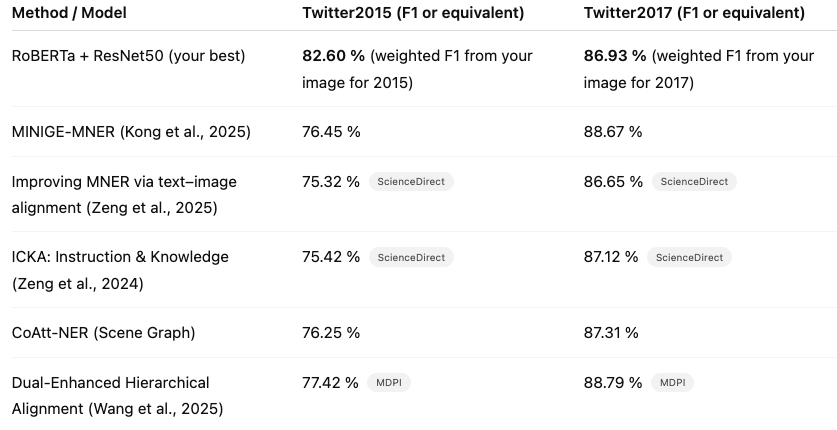
\includegraphics[width=0.85\textwidth]{literatureReview.png}
\caption{Comparative analysis of existing multimodal approaches for relationship extraction}
\label{fig:literature}
\end{figure}

Attention-based multimodal models introduced significant improvements by enabling selective integration of visual and textual features. Approaches employing visual attention guided by textual queries demonstrated enhanced ability to focus on image regions relevant to mentioned entities. Co-attention mechanisms that jointly reasoned about textual and visual salience achieved further improvements by modeling bidirectional cross-modal influences. These attention-enhanced models showed particular strength in scenarios where images contained multiple entities or complex scenes requiring selective focus. The interpretability benefits of attention weights additionally facilitated analysis of how models utilized multimodal information.

Graph-based approaches modeled relationships between entities explicitly through structured representations where nodes represent entities and edges encode relationships. Graph Convolutional Networks and Graph Attention Networks operating over entity relationship graphs demonstrated effectiveness in capturing structural patterns in relationship extraction. Multimodal extensions of graph-based methods incorporated visual features as node or edge attributes, enabling visual information to influence graph-based reasoning. These approaches proved particularly suitable for extracting multiple relationships simultaneously from documents containing numerous entity mentions, though their complexity sometimes limited scalability.

Pretrained multimodal Transformer models represent the current state-of-the-art for many vision-language tasks. Models like ViLBERT, UNITER, and OSCAR pretrained on large-scale image-text pairs learn joint representations through masked modeling objectives and cross-modal alignment tasks. Fine-tuning these models on relationship extraction tasks achieves strong performance, though computational requirements for training and inference remain substantial. The reliance on region-based visual features extracted by object detectors introduces additional complexity and potential error propagation from imperfect region proposals.

Recent work has explored prompt-based and few-shot learning approaches that reformulate relationship extraction as text generation or natural language inference tasks. These methods leverage the language understanding capabilities of large pretrained models while requiring minimal task-specific training. However, their application to multimodal settings remains less explored compared to text-only scenarios. The effectiveness of different approaches varies across datasets, domains, and relationship types, with no single method universally dominating all contexts. This variability motivates continued investigation of fusion strategies, architectures, and training procedures tailored to specific application characteristics.

\section{Research Gap Identification}

Despite substantial progress in multimodal learning and relationship extraction independently, several critical gaps persist in current research that this thesis addresses. First, while numerous studies have explored multimodal Named Entity Recognition, the specific task of multimodal relationship extraction in social media contexts remains comparatively under-investigated. Existing work has predominantly focused on entity identification rather than the more complex challenge of classifying semantic relationships between entity pairs using both textual and visual evidence. The unique characteristics of social media data including brevity, informality, and tight integration of text and images necessitate specialized approaches beyond direct application of methods designed for longer documents or formal text.

Second, comparative evaluation of fusion strategies specifically for social media relationship extraction remains limited. While early fusion, late fusion, and attention-based approaches have been studied in other multimodal contexts, systematic comparison of their effectiveness for capturing entity relationships in tweets is lacking. The optimal fusion strategy may differ from other tasks due to the specific nature of how social media users integrate visual and textual content. Understanding which fusion mechanisms best leverage complementary cross-modal information for relationship understanding represents an important research question.

Third, most existing multimodal relationship extraction work employs region-based visual features extracted through object detection models, introducing complexity and potential error propagation. Exploring alternative visual encoding approaches such as whole-image features from CNNs or patch-based features from Vision Transformers represents an under-explored direction. The trade-offs between different visual feature extraction strategies for social media images specifically designed for relationship extraction merit investigation.

Fourth, interpretability and analysis of what multimodal models learn about entity relationships receives limited attention compared to performance optimization. Understanding how visual and textual features contribute to relationship predictions, what types of relationships benefit most from multimodal integration, and when models fail to effectively leverage cross-modal information represents valuable knowledge for both improving systems and understanding multimodal communication. Systematic error analysis and qualitative investigation remain underrepresented in current literature.

Finally, while pretrained vision-language models achieve impressive results on various tasks, their application to relationship extraction specifically in noisy social media contexts with domain-specific challenges requires further exploration. The extent to which large-scale pretraining on web data transfers to Twitter's unique linguistic and visual characteristics, and whether domain-adaptive pretraining or fine-tuning strategies could improve performance, represents open questions. Additionally, investigating more parameter-efficient approaches that balance performance with computational feasibility for practical deployment remains an important consideration often overshadowed by pursuit of maximum performance regardless of resource requirements. This research addresses these gaps through systematic investigation of multimodal fusion strategies, comprehensive evaluation on standard benchmarks, and detailed analysis of model behavior and performance characteristics.

\chapter{Theoretical Framework}

\section{Overview of Multimodal Deep Learning}

Multimodal deep learning represents a paradigm that extends traditional machine learning beyond single-modality processing to handle heterogeneous data sources that naturally occur in real-world scenarios. The fundamental premise underlying multimodal learning acknowledges that intelligent systems must integrate information from multiple sensory channels to achieve comprehensive understanding comparable to human perception and cognition. In natural human communication, meaning emerges not solely from spoken or written words, but through integration of verbal content, visual cues, auditory signals, gestures, and contextual information. Similarly, effective artificial intelligence systems must develop capabilities to process and synthesize diverse information streams coherently.

The theoretical foundation of multimodal deep learning builds upon several core principles that distinguish it from unimodal approaches. The complementarity principle posits that different modalities capture distinct aspects of underlying phenomena, with each modality providing unique information not fully contained in others. For instance, in social media posts, textual content conveys explicit semantic content and linguistic structure, while accompanying images provide visual context, spatial relationships, and perceptual details difficult to articulate verbally. Effective multimodal systems leverage this complementarity to achieve more complete understanding than any single modality enables.

The redundancy principle recognizes that multiple modalities often convey overlapping information through different channels, providing robustness against noise, missing data, and ambiguity in individual modalities. When one modality contains corrupted or incomplete information, redundant information in other modalities enables the system to maintain accurate predictions. This redundancy additionally facilitates cross-modal verification where consistency or inconsistency across modalities provides signals about information reliability. In social media analysis, cross-modal consistency helps identify authentic content while inconsistencies may indicate manipulated or misleading information.

The interaction principle emphasizes that relationships between modalities carry information beyond what individual modalities contain independently. Cross-modal correlations, temporal synchronization, and semantic alignment between modalities provide additional signals that multimodal systems can exploit. For example, the specific combination of textual sentiment and visual expressions may indicate sarcasm or irony not apparent from either modality alone. Learning to model these cross-modal interactions represents a central challenge in multimodal deep learning requiring sophisticated architectural designs and training strategies.

Multimodal representation learning aims to discover joint embeddings that capture semantic content shared across modalities while preserving modality-specific characteristics. Various approaches exist including shared representations where all modalities map to a common space, coordinated representations where separate embeddings maintain alignment through learned relationships, and hierarchical representations that capture both low-level modality-specific features and high-level shared concepts. The choice of representation strategy depends on task requirements, data characteristics, and the nature of cross-modal relationships in specific application domains.

Multimodal fusion strategies determine when and how to combine information from different modalities during processing. Early fusion integrates raw or lightly processed features from multiple modalities at input stages, enabling the model to learn joint patterns from the beginning. Late fusion processes each modality independently through specialized pathways before combining high-level representations or decisions. Hybrid fusion employs intermediate integration at multiple processing stages, balancing benefits of both approaches. The optimal fusion strategy varies across tasks, with relationship extraction in social media benefiting from approaches that enable rich cross-modal interaction while respecting the distinct characteristics of textual and visual data.

\section{Representation Learning for Text and Image Modalities}

Representation learning constitutes the foundation upon which modern deep learning systems build their understanding of data. The core objective involves automatically discovering meaningful features from raw inputs through hierarchical transformations learned from training data rather than relying on manually engineered features. For multimodal systems handling both text and images, developing effective representations for each modality individually while enabling cross-modal integration presents fundamental challenges requiring careful architectural design.

Textual representation learning has evolved substantially from simple bag-of-words and TF-IDF approaches to sophisticated contextualized embeddings. Early word embedding methods like Word2Vec and GloVe learned static vector representations where each word mapped to a fixed point in semantic space regardless of context. While capturing semantic similarities and analogical relationships, static embeddings failed to represent polysemy where word meanings vary across contexts. The advent of contextualized embeddings through models like ELMo, BERT, and GPT addressed this limitation by computing context-dependent representations where the same word receives different embeddings based on surrounding text.

Transformer-based language models employ self-attention mechanisms to compute representations that capture complex dependencies across entire sequences. Each token's representation incorporates weighted contributions from all other tokens, with attention weights learned to focus on relevant context. Multiple attention heads capture different types of linguistic relationships simultaneously, while stacked Transformer layers build increasingly abstract representations. Pretraining on massive text corpora through objectives like masked language modeling enables these models to learn general linguistic knowledge transferable to downstream tasks through fine-tuning.

For social media text specifically, representation learning faces unique challenges due to informal language, domain-specific terminology, and creative linguistic expressions. Specialized tokenization strategies handle hashtags, mentions, emojis, and unconventional word boundaries. Character-level or subword tokenization improves robustness to spelling variations and out-of-vocabulary terms. Domain-adaptive pretraining on social media corpora helps models learn representations capturing platform-specific linguistic patterns. Entity-aware encoding incorporates entity type information and boundary markers to enhance entity-centric tasks like relationship extraction.

Visual representation learning through Convolutional Neural Networks implements a hierarchical processing pipeline analogous to biological visual systems. Early convolutional layers detect simple patterns like edges, corners, and textures through learned filters applied across spatial locations. Pooling operations provide translation invariance and dimensionality reduction. Deeper layers combine lower-level features to recognize increasingly complex patterns including object parts, whole objects, and scene-level semantics. This hierarchical composition enables CNNs to learn feature representations optimized for specific visual recognition tasks through supervised training.

ResNet architectures enhance visual representation learning through residual connections that enable training of very deep networks. The residual learning framework reformulates layers as learning residual functions with reference to layer inputs rather than learning unreferenced functions. Skip connections allow gradients to flow directly through many layers, mitigating vanishing gradient problems. This architecture enables networks to learn identity mappings when additional depth proves unnecessary while leveraging depth for complex pattern recognition when beneficial. The resulting deep representations capture rich semantic information about visual content including objects, scenes, activities, and attributes.

Transfer learning plays a crucial role in visual representation learning for specialized domains like social media images. Pretraining on large-scale datasets like ImageNet provides models with general-purpose visual features recognizing common objects, textures, and patterns. Fine-tuning pretrained models on domain-specific data adapts these representations to task-specific visual characteristics. For social media relationship extraction, pretrained visual encoders provide features capturing objects, people, locations, and activities visible in tweet images, which fusion mechanisms integrate with textual entity mentions to understand relationships.

\section{Mathematical Foundations of Relationship Extraction}

Relationship extraction can be formalized as a supervised classification problem operating over entity pairs within textual and visual contexts. Given a dataset $D = \{(x_i, y_i)\}_{i=1}^N$ where $x_i$ represents an input instance and $y_i \in \{r_1, r_2, ..., r_K\}$ denotes one of $K$ possible relationship types, the objective involves learning a function $f: X \rightarrow Y$ that accurately predicts relationship labels for unseen instances. In the multimodal setting relevant to social media, each input instance $x_i = (t_i, v_i, e_i^1, e_i^2)$ comprises textual content $t_i$, visual content $v_i$, and two entity mentions $e_i^1$ and $e_i^2$ whose relationship requires classification.

The textual component $t_i$ consists of a sequence of tokens $t_i = [w_1, w_2, ..., w_L]$ where $L$ represents sequence length. Entity mentions $e_i^1$ and $e_i^2$ are characterized by their positions within the sequence, typically marked through special tokens or position embeddings. A textual encoder $f_{text}: T \rightarrow \mathbb{R}^{d_{text}}$ maps the token sequence to a fixed-dimensional representation capturing semantic content and entity-specific context. For Transformer-based encoders, this involves computing contextualized embeddings through multi-head self-attention:

\begin{equation}
\text{Attention}(Q, K, V) = \text{softmax}\left(\frac{QK^T}{\sqrt{d_k}}\right)V
\end{equation}

where $Q$, $K$, and $V$ represent query, key, and value matrices derived from input embeddings, and $d_k$ denotes the dimension of key vectors. Multiple attention heads compute diverse attention patterns that are concatenated and projected to produce contextualized representations.

The visual component $v_i$ represents an image associated with the text. A visual encoder $f_{vis}: V \rightarrow \mathbb{R}^{d_{vis}}$ extracts a feature representation from the image. For CNN-based encoders like ResNet, this involves hierarchical feature extraction through convolutional layers, with the final representation typically taken from a global average pooling layer before classification:

\begin{equation}
h_{vis} = \text{GlobalAvgPool}(\text{ResNet}(v_i))
\end{equation}

This produces a $d_{vis}$-dimensional vector capturing high-level semantic content of the image.

The fusion mechanism combines textual and visual representations to produce a joint representation suitable for relationship classification. For concatenation-based fusion, the simplest approach directly concatenates modality-specific features:

\begin{equation}
h_{joint} = [h_{text}; h_{vis}]
\end{equation}

More sophisticated fusion strategies employ learned transformations. Feature-wise Linear Modulation applies affine transformations conditioned on one modality to features from another modality:

\begin{equation}
\gamma = W_{\gamma}h_{vis} + b_{\gamma}, \quad \beta = W_{\beta}h_{vis} + b_{\beta}
\end{equation}
\begin{equation}
h_{fused} = (1 + \gamma) \odot h_{text} + \beta
\end{equation}

where $\odot$ denotes element-wise multiplication, and $W_{\gamma}$, $W_{\beta}$ are learnable weight matrices. This enables visual features to modulate how textual features are processed, creating rich cross-modal interactions.

Attention-based fusion computes weighted combinations where one modality guides which aspects of the other modality receive emphasis:

\begin{equation}
\alpha = \text{softmax}(W_a[h_{text}; h_{vis}])
\end{equation}
\begin{equation}
h_{fused} = \alpha_1 h_{text} + \alpha_2 h_{vis}
\end{equation}

The final classification layer maps the fused representation to relationship label probabilities:

\begin{equation}
p(y|x) = \text{softmax}(W_{cls}h_{fused} + b_{cls})
\end{equation}

where $W_{cls}$ and $b_{cls}$ are learnable parameters.

Training optimizes parameters to minimize cross-entropy loss between predicted and true relationship labels:

\begin{equation}
\mathcal{L} = -\frac{1}{N}\sum_{i=1}^N \sum_{k=1}^K y_{ik} \log p(y_k|x_i)
\end{equation}

where $y_{ik}$ indicates whether instance $i$ belongs to class $k$. Regularization terms may be added to prevent overfitting and encourage desired properties in learned representations.

\section{Transformer Mechanisms: Self-Attention and Contextual Encoding}

The Transformer architecture revolutionized sequence modeling by replacing recurrent mechanisms with self-attention, enabling parallel processing while capturing long-range dependencies effectively. The core innovation involves computing attention weights that determine each position's relevance to every other position in a sequence, allowing dynamic focus on pertinent context regardless of distance. This mechanism proves particularly valuable for relationship extraction where understanding how entities relate requires attending to relevant portions of potentially long textual contexts.

Self-attention operates by transforming input embeddings into three different representations: queries, keys, and values. For an input sequence with embeddings $X = [x_1, ..., x_L] \in \mathbb{R}^{L \times d}$, these projections are computed as:

\begin{equation}
Q = XW^Q, \quad K = XW^K, \quad V = XW^V
\end{equation}

where $W^Q, W^K, W^V \in \mathbb{R}^{d \times d_k}$ are learnable projection matrices. The attention mechanism then computes how much each position should attend to every other position by taking dot products between queries and keys, scaling by the square root of dimension for numerical stability, and applying softmax to obtain attention weights:

\begin{equation}
A = \text{softmax}\left(\frac{QK^T}{\sqrt{d_k}}\right) \in \mathbb{R}^{L \times L}
\end{equation}

These attention weights determine how to aggregate value vectors to produce output representations:

\begin{equation}
\text{SelfAttention}(X) = AV
\end{equation}

Multi-head attention extends this mechanism by computing multiple attention patterns in parallel, each potentially capturing different types of relationships. With $h$ attention heads, the input undergoes $h$ separate attention computations with distinct parameter matrices:

\begin{equation}
\text{head}_i = \text{Attention}(XW_i^Q, XW_i^K, XW_i^V)
\end{equation}

The outputs from all heads are concatenated and projected through a final linear layer:

\begin{equation}
\text{MultiHead}(X) = \text{Concat}(\text{head}_1, ..., \text{head}_h)W^O
\end{equation}

This multi-head structure enables the model to jointly attend to information from different representation subspaces at different positions, capturing diverse linguistic phenomena simultaneously.

Position encodings inject sequential information into the otherwise permutation-invariant attention mechanism. Sinusoidal position encodings use trigonometric functions of different frequencies:

\begin{equation}
PE_{(pos, 2i)} = \sin(pos / 10000^{2i/d})
\end{equation}
\begin{equation}
PE_{(pos, 2i+1)} = \cos(pos / 10000^{2i/d})
\end{equation}

where $pos$ denotes position and $i$ denotes dimension. These encodings are added to input embeddings, allowing the model to distinguish different positions and learn position-dependent patterns.

Layer normalization and residual connections stabilize training of deep Transformer networks. Each sub-layer employs a residual connection followed by layer normalization:

\begin{equation}
\text{Output} = \text{LayerNorm}(X + \text{Sublayer}(X))
\end{equation}

Feed-forward networks within each Transformer layer apply position-wise transformations:

\begin{equation}
\text{FFN}(x) = \max(0, xW_1 + b_1)W_2 + b_2
\end{equation}

For relationship extraction, Transformer encoders produce contextualized representations where each token's embedding incorporates information from the entire sequence. Entity representations can be extracted by pooling over entity mention spans or using special entity marker tokens. These contextualized entity representations capture not just the entity itself but also surrounding context relevant to understanding its relationships with other entities.

\section{Residual Learning and Image Feature Abstraction using ResNet}

Residual learning addresses fundamental challenges in training very deep neural networks that conventional architectures encounter. As network depth increases, optimization becomes increasingly difficult due to vanishing or exploding gradients where error signals diminish or amplify exponentially as they propagate backward through many layers. Additionally, empirical observations revealed a degradation problem where deeper plain networks exhibited higher training error than shallower counterparts, suggesting optimization difficulty rather than overfitting as the primary limitation.

The residual learning framework reformulates the learning problem by introducing skip connections that add a layer's input directly to its output. Instead of learning an unreferenced mapping $H(x)$, residual blocks learn a residual function $F(x) = H(x) - x$ with the final output being $H(x) = F(x) + x$. This formulation hypothesizes that learning residual mappings proves easier than learning original unreferenced mappings, particularly when optimal mappings lie close to identity functions. If identity mappings are optimal, the network can simply learn to drive residual function weights toward zero rather than learning identity mappings through multiple nonlinear layers.

A residual block typically consists of two or three convolutional layers with batch normalization and ReLU activations, with the input added to the output before final activation:

\begin{equation}
y = F(x, \{W_i\}) + x
\end{equation}
\begin{equation}
\text{Output} = \text{ReLU}(y)
\end{equation}

where $F(x, \{W_i\})$ represents the residual mapping to be learned. When input and output dimensions differ, a linear projection $W_s$ applied to the shortcut connection ensures dimensional compatibility:

\begin{equation}
y = F(x, \{W_i\}) + W_s x
\end{equation}

ResNet-50 architecture organizes 50 convolutional layers into a sequence of residual blocks grouped into four stages. The network begins with a standard convolutional layer and max pooling, followed by stages containing 3, 4, 6, and 3 residual blocks respectively. Each stage operates at a different spatial resolution, with dimensions halved and channel depth doubled between stages. Within stages, residual blocks maintain consistent dimensions enabling direct skip connections, while transition blocks between stages employ projection shortcuts to handle dimensional changes.

The bottleneck design used in deeper ResNet variants employs 1x1 convolutions to reduce and restore dimensions around 3x3 convolutions, reducing computational cost while maintaining representational capacity:

\begin{equation}
F(x) = W_3(\text{ReLU}(W_2(\text{ReLU}(W_1 x))))
\end{equation}

where $W_1$ reduces dimension, $W_2$ applies 3x3 convolution, and $W_3$ restores dimension.

For multimodal relationship extraction, ResNet-50 pretrained on ImageNet serves as a powerful visual feature extractor. The network processes tweet images through its convolutional stages, producing feature maps capturing hierarchical visual patterns. Global average pooling over the final convolutional layer produces a 2048-dimensional feature vector encoding high-level semantic content. This visual representation captures objects, scenes, people, text, and spatial relationships visible in images, providing contextual information complementing textual entity mentions. Transfer learning from ImageNet pretraining enables effective feature extraction even when social media image datasets remain limited, as the pretrained weights encode general visual knowledge applicable across domains.

\section{Fusion Architecture for Joint Embedding}

The fusion architecture determines how textual and visual representations combine to produce joint embeddings suitable for relationship classification. Effective fusion mechanisms must balance several competing objectives including preserving complementary information from both modalities, learning meaningful cross-modal interactions, maintaining computational efficiency, and enabling interpretability of how different modalities contribute to predictions. The choice of fusion strategy significantly impacts model performance, with optimal approaches varying based on task characteristics and data properties.

Concatenation-based fusion represents the conceptually simplest approach where modality-specific representations are directly concatenated before feeding into classification layers. Given textual features $h_{text} \in \mathbb{R}^{d_t}$ and visual features $h_{vis} \in \mathbb{R}^{d_v}$, concatenation produces:

\begin{equation}
h_{concat} = [h_{text}; h_{vis}] \in \mathbb{R}^{d_t + d_v}
\end{equation}

This concatenated representation passes through fully connected layers that learn to weight and combine features:

\begin{equation}
h_{joint} = \text{ReLU}(W_{fc}h_{concat} + b_{fc})
\end{equation}

While simple and computationally efficient, pure concatenation provides limited flexibility for modeling complex cross-modal interactions since it treats both modalities symmetrically and relies entirely on subsequent layers to discover relevant cross-modal patterns.

Feature-wise Linear Modulation introduces asymmetric conditioning where one modality modulates features from another through learned affine transformations. This approach proves particularly effective when one modality provides contextual information that should influence processing of another modality. For visual conditioning of textual features:

\begin{equation}
\gamma = \text{ReLU}(W_{\gamma}h_{vis} + b_{\gamma})
\end{equation}
\begin{equation}
\beta = \text{ReLU}(W_{\beta}h_{vis} + b_{\beta})
\end{equation}
\begin{equation}
h_{modulated} = \gamma \odot h_{text} + \beta
\end{equation}

The scale parameter $\gamma$ and shift parameter $\beta$ are conditioned on visual features, enabling images to adaptively influence how textual features contribute to final predictions. This mechanism creates rich cross-modal interactions while remaining computationally efficient and interpretable.

Attention-based fusion employs learned attention mechanisms to dynamically weight contributions from different modalities. Cross-modal attention computes attention weights for one modality conditioned on the other:

\begin{equation}
e = W_e h_{vis} + b_e
\end{equation}
\begin{equation}
\alpha_i = \frac{\exp(e^T h_{text}^i)}{\sum_j \exp(e^T h_{text}^j)}
\end{equation}
\begin{equation}
h_{attended} = \sum_i \alpha_i h_{text}^i
\end{equation}

This allows visual features to guide which aspects of textual representation receive emphasis, particularly useful when text contains multiple entities or complex linguistic structures requiring selective focus.

Bilinear fusion computes pairwise interactions between all dimensions of modality-specific representations through a learned weight tensor:

\begin{equation}
h_{bilinear} = h_{text}^T W_{bilinear} h_{vis}
\end{equation}

While theoretically powerful for capturing complex interactions, bilinear fusion's computational and memory requirements scale quadratically with feature dimensions, often necessitating low-rank approximations or factorized implementations for practical deployment.

The proposed architecture for multimodal relationship extraction employs a hybrid fusion strategy combining multiple mechanisms. Textual features from RoBERTa and visual features from ResNet-50 first undergo projection to a common dimension. FiLM-based modulation enables cross-modal conditioning, followed by concatenation and attention mechanisms that adaptively weight modality contributions. This multi-stage fusion enables the model to capture both fine-grained feature-level interactions through FiLM and coarse-grained modality-level weighting through attention, balancing expressiveness with computational efficiency.

\section{Evaluation Metrics: Accuracy, Precision, Recall, F1-Score}

Rigorous evaluation of relationship extraction systems requires comprehensive metrics that capture different aspects of model performance. The choice of evaluation metrics depends on task characteristics, class distribution, and application requirements. For relationship extraction, where multiple relationship types exist with potentially imbalanced distributions, relying solely on accuracy proves insufficient, necessitating additional metrics that account for precision-recall trade-offs and class-specific performance.

Accuracy measures the proportion of correct predictions across all instances:

\begin{equation}
\text{Accuracy} = \frac{\text{Number of Correct Predictions}}{\text{Total Number of Predictions}} = \frac{TP + TN}{TP + TN + FP + FN}
\end{equation}

where $TP$, $TN$, $FP$, and $FN$ denote true positives, true negatives, false positives, and false negatives respectively. While intuitive and commonly reported, accuracy can be misleading for imbalanced datasets where a naive classifier predicting only the majority class achieves high accuracy despite poor practical utility.

Precision quantifies the proportion of predicted positive instances that are actually positive, measuring the model's ability to avoid false positives:

\begin{equation}
\text{Precision} = \frac{TP}{TP + FP}
\end{equation}

High precision indicates that when the model predicts a particular relationship type, this prediction is likely correct. Precision proves particularly important in applications where false positives incur significant costs or where users require high confidence in positive predictions.

Recall, also termed sensitivity, measures the proportion of actual positive instances correctly identified by the model:

\begin{equation}
\text{Recall} = \frac{TP}{TP + FN}
\end{equation}

High recall indicates comprehensive capture of true positive instances with few missed detections. Recall assumes priority in applications where missing positive instances incurs greater cost than occasional false alarms, such as medical diagnosis or security-critical systems.

The F1-score provides a harmonic mean of precision and recall, balancing both metrics into a single value:

\begin{equation}
\text{F1} = 2 \times \frac{\text{Precision} \times \text{Recall}}{\text{Precision} + \text{Recall}} = \frac{2TP}{2TP + FP + FN}
\end{equation}

The harmonic mean ensures that F1-score achieves high values only when both precision and recall are high, preventing inflation from strong performance on just one metric. F1-score proves particularly useful for comparing models when both precision and recall matter and no clear priority exists between them.

For multi-class relationship extraction, metrics can be computed at micro, macro, and weighted levels. Micro-averaging aggregates contributions from all classes before computing metrics, treating each instance equally:

\begin{equation}
\text{Precision}_{micro} = \frac{\sum_{k=1}^K TP_k}{\sum_{k=1}^K (TP_k + FP_k)}
\end{equation}

Macro-averaging computes metrics independently for each class then averages across classes, treating each class equally regardless of size:

\begin{equation}
\text{Precision}_{macro} = \frac{1}{K}\sum_{k=1}^K \frac{TP_k}{TP_k + FP_k}
\end{equation}

Weighted-averaging computes per-class metrics then averages weighted by class support, accounting for class imbalance:

\begin{equation}
\text{Precision}_{weighted} = \frac{1}{N}\sum_{k=1}^K n_k \frac{TP_k}{TP_k + FP_k}
\end{equation}

where $n_k$ denotes the number of true instances in class $k$ and $N = \sum_k n_k$ represents total instances.

For relationship extraction evaluation, micro-averaged F1-score serves as the primary metric as it provides a balanced assessment of overall performance across all relationship types while appropriately weighting performance on frequent relationships. Macro-averaged metrics additionally provide insight into performance across relationship types regardless of frequency, revealing whether models perform consistently or exhibit wide performance variation. Per-class precision, recall, and F1-scores enable detailed analysis identifying which relationship types prove most challenging and where improvements are most needed. Comprehensive evaluation reports these metrics across multiple aggregation levels, providing a complete picture of model capabilities and limitations that informs both research insights and practical deployment decisions.

\chapter{Methodology}

\section{Research Design}

This research employs an experimental design methodology grounded in empirical evaluation of deep learning models for multimodal relationship extraction in Twitter data. The investigation follows a systematic approach encompassing dataset preparation, model development, training, evaluation, and comparative analysis. The research design adheres to principles of reproducibility, ensuring that all experimental procedures, hyperparameter configurations, and evaluation protocols are documented comprehensively to enable verification and extension by the research community.

The methodological framework operates through several interconnected phases. The initial phase involves comprehensive data collection, preprocessing, and preparation of Twitter2015 and Twitter2017 benchmark datasets. These datasets provide standardized evaluation environments enabling fair comparison with existing approaches and establishing baseline performance metrics. The preprocessing phase addresses challenges specific to social media data including handling informal language, special tokens, hashtags, mentions, and ensuring proper alignment between textual content and accompanying images.

The model development phase focuses on implementing and integrating multiple architectural components. Visual feature extraction employs ResNet-50 pretrained on ImageNet, leveraging transfer learning to obtain robust visual representations despite limited domain-specific training data. Textual encoding utilizes RoBERTa-large, a state-of-the-art Transformer-based language model pretrained on diverse text corpora. The fusion mechanism implements FiLM-based conditioning that enables rich cross-modal interactions between visual and textual modalities. This modular architecture allows systematic investigation of individual component contributions through ablation studies.

The training phase employs supervised learning with cross-entropy loss, optimizing model parameters through gradient descent with adaptive learning rate scheduling. Multiple training strategies are explored including different batch sizes, learning rates, optimization algorithms, and regularization techniques. Data augmentation applies transformations to both visual and textual inputs to improve generalization and reduce overfitting. The validation set guides hyperparameter tuning and early stopping decisions, preventing overfitting while maximizing performance on held-out test data.

The evaluation phase measures model performance using multiple metrics including accuracy, precision, recall, and F1-score computed at micro, macro, and weighted averaging levels. Comparative analysis examines performance relative to baseline approaches including text-only models, vision-only models, and alternative multimodal fusion strategies. Ablation studies systematically remove or modify individual components to quantify their contributions to overall performance. Error analysis and qualitative investigation provide insights into model behavior, failure modes, and opportunities for improvement.

The experimental design incorporates rigorous controls to ensure validity and reliability of findings. Fixed random seeds ensure reproducibility of results across multiple runs. Consistent train-validation-test splits prevent data leakage and enable fair comparison across different model configurations. Statistical significance testing where applicable provides confidence in observed performance differences. Comprehensive documentation of all experimental details including software versions, hardware specifications, and hyperparameter settings facilitates reproducibility and enables other researchers to build upon this work.

\section{Dataset Description}

\subsection{Twitter2015 Dataset}

The Twitter2015 dataset represents one of the benchmark collections for evaluating multimodal Named Entity Recognition systems on social media data. This dataset was constructed by collecting tweets that contain both textual content and accompanying images, with manual annotation of named entities and their types. The dataset reflects the authentic characteristics of Twitter communication including informal language, hashtags, user mentions, URLs, and the tight integration of visual and textual content that defines contemporary social media interaction.

The Twitter2015 dataset comprises a total of 4,290 tweets divided into training, validation, and test sets following standard data splitting protocols. The training set contains 3,257 tweets providing sufficient examples for supervised learning while maintaining computational feasibility. The validation set includes 516 tweets used for hyperparameter tuning, model selection, and early stopping decisions during training. The test set consists of 517 tweets held out completely from the training process to provide unbiased evaluation of final model performance. This partitioning ensures that models encounter genuinely unseen examples during evaluation, providing realistic assessment of generalization capabilities.

Named entities in the Twitter2015 dataset are annotated according to four primary categories: Person, Location, Organization, and Other. The Person category includes individuals, celebrities, public figures, and character references appearing in tweets. The Location category encompasses geographic entities including cities, countries, landmarks, and spatial references. The Organization category covers companies, institutions, government bodies, sports teams, and other organizational entities. The Other category captures miscellaneous named entities not fitting cleanly into the three primary categories. Entities are marked using BIO tagging scheme where B-prefixes indicate beginning tokens, I-prefixes indicate inside tokens, and O denotes non-entity tokens.

Each tweet in the dataset includes several components essential for multimodal processing. The textual content preserves original tweet formatting including hashtags, mentions, and special characters, maintaining authenticity of social media language. Image identifiers link tweets to corresponding image files, enabling retrieval of visual content during model training and evaluation. Entity annotations specify the positions and types of named entities within each tweet, providing ground truth labels for supervised learning. The dataset additionally includes metadata such as tweet identifiers, timestamps, and user information, though privacy considerations limit the availability of certain sensitive attributes.

The visual content in Twitter2015 exhibits substantial diversity reflecting the varied purposes for which users share images on social media. Images range from personal photographs capturing social events and daily activities to news photographs depicting current events and public figures. Memes, screenshots, infographics, and promotional content appear frequently. Image quality varies considerably from professional photography to low-resolution mobile captures. This heterogeneity presents challenges for visual feature extraction but also ensures that models trained on this data develop robustness to the diverse visual content encountered in real-world social media streams.

\subsection{Twitter2017 Dataset}

The Twitter2017 dataset extends the earlier Twitter2015 collection with an expanded set of tweets and refinements to annotation procedures based on lessons learned from the initial dataset construction. This dataset maintains consistency with Twitter2015 in terms of entity categories and annotation scheme, enabling combined training and direct performance comparison across datasets. The Twitter2017 collection reflects evolving patterns in social media usage including increased multimedia integration and changing linguistic conventions.

The Twitter2017 dataset contains approximately 3,373 tweets split into training, validation, and test partitions. The training set provides 1,975 annotated tweets for model learning, while the validation set includes 608 tweets for development-time evaluation and hyperparameter optimization. The test set comprises 790 tweets reserved exclusively for final performance assessment. Although smaller in total size compared to Twitter2015, the Twitter2017 dataset offers value through its more recent content reflecting contemporary social media practices and its utility for evaluating cross-dataset generalization when models trained on one dataset are tested on the other.

Entity annotations in Twitter2017 follow the same four-category taxonomy as Twitter2015, using identical BIO tagging conventions to ensure compatibility and facilitate joint training scenarios. The annotation quality in Twitter2017 benefits from refined guidelines addressing ambiguous cases encountered during Twitter2015 annotation. Inter-annotator agreement metrics indicate high consistency in entity boundary detection and type classification, providing confidence in the reliability of ground truth labels. Double annotation with adjudication of disagreements further enhances annotation quality, reducing label noise that could impair model training.

The multimodal nature of Twitter2017 manifests through strong coupling between textual and visual content. Many tweets explicitly reference visual elements in accompanying images, creating dependencies where full understanding requires processing both modalities. For instance, location entities mentioned textually may correspond to landmarks visible in images, while person entities referenced by name may appear visually through photographs or recognizable contexts. This cross-modal grounding provides opportunities for multimodal models to leverage complementary information but also creates challenges when misalignment occurs between textual mentions and visual content.

Both Twitter2015 and Twitter2017 datasets present characteristic challenges that motivate multimodal approaches. Entity mentions frequently suffer from ambiguity resolvable through visual context. Abbreviated entity references and informal language complicate text-only recognition. The visual grounding of entities in images provides disambiguating evidence and additional context. However, not all images contain entities mentioned in text, and some tweets include images serving primarily aesthetic or emotional purposes rather than informational content directly related to entity mentions. These complexities make the datasets valuable testbeds for evaluating multimodal relationship extraction systems capable of leveraging cross-modal information when beneficial while maintaining robustness when modalities misalign.

\section{Data Preprocessing}

\subsection{Text Cleaning and Tokenization}

Text preprocessing for social media data requires specialized handling to address the unique characteristics of Twitter language while preserving information-bearing elements that standard text cleaning might inappropriately remove. The preprocessing pipeline begins with careful normalization that maintains the authentic nature of social media communication while enabling effective processing by neural language models. Unlike formal text where aggressive cleaning and standardization prove beneficial, social media preprocessing must balance noise reduction with preservation of meaningful linguistic signals.

The tokenization strategy employs the RoBERTa tokenizer based on byte-pair encoding, which provides several advantages for processing Twitter text. Subword tokenization handles out-of-vocabulary terms gracefully by breaking unknown words into known subword units, addressing the prevalence of neologisms, creative spellings, and domain-specific terminology in social media. The tokenizer preserves special characters and punctuation that may carry semantic meaning in informal contexts. Hashtags are retained as complete tokens when possible, though the tokenizer may split very long concatenated hashtags into constituent parts. User mentions prefixed with the @ symbol are preserved to maintain reference information, though specific usernames may be replaced with generic mention tokens for privacy considerations.

Entity markers inserted during preprocessing play a crucial role in helping the model identify entity mentions and their boundaries within tokenized sequences. Special tokens demarcate entity spans, with different marker types potentially indicating entity categories when available from annotations. For instance, an entity mention might be enclosed between [E1] and [/E1] tokens for the first entity in a relationship extraction instance, while [E2] and [/E2] tokens mark the second entity. These markers enable the model to learn entity-specific representations that capture contextual information surrounding entities relevant to relationship classification.

URL normalization replaces specific URLs with a generic URL token since the particular web addresses typically carry minimal information for entity recognition while introducing substantial vocabulary expansion. Similarly, numbers may be normalized to generic number tokens to reduce vocabulary size and improve generalization, though this decision requires careful consideration as some numbers carry semantic importance. Emoji handling preserves these graphical symbols as they often convey sentiment and emphasis important for understanding social media communication. The RoBERTa tokenizer's vocabulary includes many common emoji, enabling their representation as discrete tokens.

Sequence length management addresses the variable length of tweets and the fixed input size requirements of Transformer models. While Twitter's character limit naturally constrains tweet length, tokenization can produce sequences exceeding model capacity due to subword splitting. Truncation strategies handle overly long sequences, typically retaining initial portions where entity mentions concentrate while discarding trailing content. Padding ensures uniform sequence lengths within batches, with special padding tokens added to shorter sequences. Attention masks distinguish actual content tokens from padding, ensuring that padding tokens do not influence model computations.

Lowercasing decisions require nuance in social media contexts. Traditional text processing often converts all text to lowercase to reduce vocabulary size and improve generalization. However, capitalization in tweets sometimes carries meaningful information, particularly for entity recognition where proper nouns traditionally appear capitalized. The RoBERTa model processes text in its original case during pretraining, and maintaining case information during fine-tuning proves beneficial for preserving entity-relevant signals despite inconsistent capitalization patterns in social media.

\subsection{Image Normalization and Feature Extraction}

Image preprocessing transforms raw tweet images into normalized tensors suitable for processing by ResNet-50 while applying augmentation techniques that improve model robustness and generalization. The preprocessing pipeline addresses the substantial heterogeneity in social media images including varied resolutions, aspect ratios, color characteristics, and quality levels. Standardization ensures that all images undergo consistent transformations producing inputs matching the specifications required by pretrained ResNet models.

Resizing operations transform images to fixed dimensions matching ResNet-50 input requirements. The standard approach resizes images to 224x224 pixels, the native input resolution for ImageNet-pretrained ResNet models. For images with aspect ratios differing substantially from square, direct resizing to square dimensions introduces distortion potentially degrading visual information. Alternative strategies employ resizing to intermediate dimensions followed by center cropping to obtain the target 224x224 size, preserving aspect ratios while focusing on central image regions assumed to contain primary visual content.

Color normalization applies channel-wise mean subtraction and standard deviation division using statistics computed from the ImageNet training set. This normalization ensures that image pixel value distributions match those encountered during ResNet pretraining, facilitating effective transfer learning. The specific normalization values are mean=[0.485, 0.456, 0.406] and std=[0.229, 0.224, 0.225] for red, green, and blue channels respectively. This preprocessing transforms pixel values from the original 0-255 range to standardized distributions centered near zero.

Data augmentation during training applies random transformations that create variation in training examples without requiring additional labeled data. Random horizontal flipping with 50 percent probability introduces viewpoint variations, helping models develop invariance to left-right orientations. Random cropping selects variable portions of images, encouraging the model to learn robust features not dependent on specific spatial configurations. Color jittering randomly perturbs brightness, contrast, saturation, and hue within constrained ranges, improving robustness to illumination and color balance variations. These augmentations apply only during training, while validation and test images undergo deterministic preprocessing to ensure reproducible evaluation.

Missing image handling addresses cases where image files corresponding to tweets cannot be located or loaded due to data collection issues or file corruption. When images are unavailable, the system generates blank placeholder images maintaining the correct dimensions and channel structure. This approach enables uniform processing of all instances while preventing errors from missing data. The model learns to handle such cases through exposure during training, potentially developing strategies to rely more heavily on textual information when visual content appears uninformative.

The feature extraction process passes preprocessed images through ResNet-50, utilizing the convolutional backbone up to the global average pooling layer. This produces a 2048-dimensional feature vector for each image, capturing high-level semantic visual information learned during ImageNet pretraining. These features encode objects, scenes, textures, colors, and spatial relationships present in images. The pretrained weights remain fixed during initial training phases to leverage learned representations, though later experiments may explore fine-tuning visual encoders on task-specific data to adapt features to social media imagery characteristics.

\subsection{Handling Hashtags, Emojis, and Slang}

Social media language incorporates distinctive elements including hashtags, emojis, and slang that convey meaning through non-standard linguistic forms. Effective preprocessing must handle these elements appropriately to preserve their semantic contributions while enabling successful processing by neural language models. The strategies employed balance retention of information with practical constraints imposed by model architectures and vocabulary limitations.

Hashtags serve multiple communicative functions in Twitter, marking topics, expressing sentiment, participating in conversations, and organizing content around themes or events. A hashtag consists of the hash symbol followed by concatenated words without spaces, such as #BlackLivesMatter or #COVID19. Preprocessing handles hashtags in several ways depending on their characteristics. Short hashtags already present in the tokenizer vocabulary are retained as single tokens, preserving their atomic semantic units. Long concatenated hashtags may be segmented into constituent words through hashtag segmentation algorithms that identify likely word boundaries based on vocabulary matching and linguistic patterns.

Alternatively, hashtags can be processed by simply removing the hash symbol while preserving the text, allowing the tokenizer to split the content according to standard subword tokenization. This approach works well when hashtags consist of common words or phrases, though it loses the explicit signal that the content originated as a hashtag which may carry pragmatic meaning. Some models employ special hashtag tokens or retain the hash symbol to maintain this distinction. The optimal approach often depends on the specific characteristics of the dataset and task requirements.

Emojis represent graphical symbols conveying emotions, objects, activities, and concepts through pictographic representations. Modern Unicode standards define thousands of emoji characters covering diverse semantic categories. The RoBERTa tokenizer includes many common emoji in its vocabulary, enabling their representation as discrete tokens. When emoji appear in the vocabulary, they are tokenized as single units preserving their semantic integrity. Emoji not in the vocabulary may be broken into constituent Unicode characters or replaced with unknown tokens, potentially losing information.

Some preprocessing approaches employ emoji-to-text conversion, replacing graphical emoji with textual descriptions of their meanings, such as converting a smiling face emoji to the word "happy" or textual description "smiling face". This approach makes emoji semantics more explicit and avoids vocabulary coverage issues, though it may introduce ambiguity when single emoji map to multiple possible interpretations. The research employs the standard RoBERTa vocabulary which includes common emoji, relying on the model's learned representations to capture their meanings from pretraining exposure.

Slang, abbreviations, and informal language forms present additional challenges requiring careful consideration. Social media users frequently employ shortened forms like "bc" for "because", "ur" for "your/you're", and "tbh" for "to be honest". Domain-specific terminology and community-specific language evolve rapidly, with new terms and usages emerging continuously. The subword tokenization approach provides inherent robustness to these phenomena by breaking unknown terms into known components, though this may not capture intended meanings for highly creative linguistic expressions.

Spelling variations and intentional misspellings like "sooooo" for emphasis or "thicc" as stylistic spelling of "thick" occur frequently in social media text. The RoBERTa model's pretraining on diverse text corpora including social media provides exposure to many such variations, enabling the model to learn representations that capture their meanings despite deviations from standard spelling. Character-level or subword processing additionally helps by representing these variations through combinations of standard character sequences, providing some semantic continuity with correctly spelled variants.

\section{Feature Extraction Modules}

\subsection{Textual Feature Extraction (Transformer Encoder)}

The textual feature extraction module employs RoBERTa-large as the primary encoder for processing tweet text and producing contextualized representations suitable for relationship extraction. RoBERTa, an optimized variant of BERT, consists of 24 Transformer layers with 16 attention heads and 1024-dimensional hidden representations, totaling approximately 355 million parameters. The model was pretrained on 160GB of text data through masked language modeling, learning to predict randomly masked tokens based on surrounding context. This pretraining enables RoBERTa to capture rich linguistic knowledge including syntax, semantics, and pragmatics transferable to downstream tasks.

The input to RoBERTa consists of tokenized text with special markers indicating entity positions. The tokenization produces a sequence of token IDs corresponding to subword units in RoBERTa's vocabulary. Special tokens including [CLS] at the sequence beginning and [SEP] at the end follow BERT conventions, though their specific roles vary across tasks. Entity markers inserted during preprocessing help the model identify entity mentions and learn entity-specific representations. The input sequence undergoes embedding through learned embedding matrices that map token IDs to dense vector representations.

Position embeddings add positional information to token embeddings, enabling the model to distinguish tokens based on their sequence positions despite the permutation-invariant nature of self-attention. The combined token and position embeddings feed into the first Transformer layer. Each Transformer layer applies multi-head self-attention followed by position-wise feed-forward networks, with residual connections and layer normalization stabilizing training. The self-attention mechanism computes attention weights determining how much each token should attend to every other token, enabling the model to capture long-range dependencies and contextual relationships crucial for understanding entity mentions and their relationships.

The output from the final Transformer layer consists of contextualized embeddings for each input token, with each token's 1024-dimensional representation incorporating information from the entire sequence through multiple layers of self-attention. For relationship extraction, entity representations are extracted by pooling over entity mention spans or using representations of special entity marker tokens. These entity-specific representations capture not only the lexical content of entity mentions but also surrounding contextual information relevant to understanding relationships between entities.

Fine-tuning strategies adapt the pretrained RoBERTa model to the specific characteristics of Twitter data and relationship extraction tasks. During fine-tuning, the entire network or selected layers undergo gradient updates using labeled examples from the training set. The learning rate for fine-tuning is typically set lower than initial pretraining to preserve learned representations while adapting them to task-specific requirements. Dropout regularization applied during fine-tuning prevents overfitting to limited task-specific training data. Layer-wise learning rate decay applies progressively smaller learning rates to lower layers, making minimal modifications to early feature extractors while enabling greater adaptation in higher layers closer to task-specific outputs.

\subsection{Visual Feature Extraction (ResNet Backbone)}

Visual feature extraction employs ResNet-50, a 50-layer deep residual network pretrained on ImageNet, to process tweet images and produce high-dimensional feature representations capturing semantic visual content. The architecture consists of an initial 7x7 convolutional layer followed by max pooling, then four stages of residual blocks operating at progressively lower spatial resolutions with increasing channel depths. The four stages contain 3, 4, 6, and 3 residual blocks respectively, with each block implementing the bottleneck design using 1x1, 3x3, and 1x1 convolutions.

Preprocessed images enter the network as 224x224x3 tensors after normalization and potential augmentation. The initial convolution with stride 2 reduces spatial dimensions to 112x112 while expanding channels to 64. Max pooling further reduces resolution to 56x56. The first stage processes features at 56x56 resolution with 256 channels. The second stage operates at 28x28 resolution with 512 channels. The third stage works at 14x14 resolution with 1024 channels. The final stage produces features at 7x7 resolution with 2048 channels.

Global average pooling aggregates the final convolutional feature maps across spatial dimensions, producing a single 2048-dimensional vector summarizing visual content of the entire image. This pooling operation provides translation invariance and dimensionality reduction while preserving channel-wise semantic information. The resulting feature vector captures high-level visual concepts learned during ImageNet pretraining including object categories, scene types, textures, colors, and spatial relationships.

Transfer learning from ImageNet pretraining provides ResNet-50 with general-purpose visual representations applicable across diverse image recognition tasks. Although ImageNet training focused on object classification with 1000 categories, the learned features capture generalizable visual patterns useful for understanding social media images despite domain differences. The convolutional filters in early layers detect edges, corners, and basic textures applicable across domains. Deeper layers recognize increasingly complex patterns including object parts and whole objects that frequently appear in social media images.

The frozen feature extraction approach maintains pretrained ResNet weights without modification during initial training phases. This strategy leverages learned representations while limiting computational requirements and reducing overfitting risk on limited domain-specific training data. The frozen backbone serves purely as a feature extractor, with learned parameters residing only in subsequent fusion and classification layers. Alternative approaches involve fine-tuning ResNet weights on task-specific data, potentially adapting visual features to social media image characteristics. However, fine-tuning requires larger training sets and greater computational resources while risking overfitting. The research primarily employs frozen features based on empirical observations that fine-tuning provides minimal benefits given available training data sizes.

\section{Fusion Mechanism}

\subsection{Concatenation-based Fusion}

Concatenation-based fusion represents a straightforward baseline approach for combining textual and visual features. This strategy directly concatenates the 1024-dimensional textual representation from RoBERTa with the 2048-dimensional visual representation from ResNet-50, producing a 3072-dimensional joint representation. Mathematically, given textual features $h_t \in \mathbb{R}^{1024}$ and visual features $h_v \in \mathbb{R}^{2048}$, concatenation produces $h_c = [h_t; h_v] \in \mathbb{R}^{3072}$.

The concatenated representation passes through one or more fully connected layers that learn to weight and combine features from both modalities for relationship classification. A typical configuration employs a hidden layer with ReLU activation followed by dropout regularization before the final classification layer. The hidden layer might reduce dimensionality to 512 or 1024 units, learning a compressed joint representation that preserves information relevant to relationship extraction while discarding irrelevant variations. The mathematical formulation is:

\begin{equation}
h_{hidden} = \text{ReLU}(W_1 h_c + b_1)
\end{equation}
\begin{equation}
h_{dropped} = \text{Dropout}(h_{hidden}, p=0.1)
\end{equation}
\begin{equation}
\text{logits} = W_2 h_{dropped} + b_2
\end{equation}

where $W_1, b_1, W_2, b_2$ are learned parameters. The dropout probability $p$ controls the strength of regularization, with $p=0.1$ providing mild regularization suitable for moderately-sized models.

Concatenation-based fusion offers several advantages including simplicity, ease of implementation, and computational efficiency. The approach requires minimal additional parameters beyond the classification layers, reducing memory requirements and training time. Concatenation treats both modalities symmetrically, allowing the model to learn appropriate weighting through supervised training on task-specific data. The fully connected layers following concatenation can learn arbitrary functions of the combined features, providing flexibility to discover relevant cross-modal patterns.

However, pure concatenation exhibits limitations in modeling complex cross-modal interactions. The symmetric treatment of modalities does not account for situations where one modality dominates importance or where cross-modal dependencies require asymmetric processing. Concatenation relies entirely on subsequent layers to discover cross-modal relationships, potentially requiring deeper networks or larger parameter counts to achieve performance matching more sophisticated fusion strategies. Despite these limitations, concatenation provides a strong baseline establishing minimum expected performance for multimodal approaches.

\subsection{Attention and FiLM-based Fusion (Novel Approach)}

The proposed novel fusion approach combines Feature-wise Linear Modulation (FiLM) with attention mechanisms to enable rich cross-modal interactions while maintaining computational efficiency. This hybrid strategy leverages the complementary strengths of FiLM's fine-grained feature modulation and attention's dynamic weighting capabilities, creating a fusion architecture specifically designed for multimodal relationship extraction in social media.

The FiLM component implements visual conditioning of textual features through learned affine transformations. Visual features from ResNet-50 first undergo projection to match the dimensionality of textual features. Two separate linear transformations learn scale ($\gamma$) and shift ($\beta$) parameters conditioned on visual content:

\begin{equation}
h_v^{proj} = W_{proj} h_v + b_{proj}
\end{equation}
\begin{equation}
\gamma = W_{\gamma} h_v^{proj} + b_{\gamma}
\end{equation}
\begin{equation}
\beta = W_{\beta} h_v^{proj} + b_{\beta}
\end{equation}

These parameters modulate textual features through element-wise scaling and shifting:

\begin{equation}
h_t^{modulated} = (1 + \gamma) \odot h_t + \beta
\end{equation}

where $\odot$ denotes element-wise multiplication. This modulation enables visual information to influence how textual features contribute to relationship predictions. When images contain relevant visual context, the learned modulation can amplify or suppress specific textual feature dimensions accordingly. The additive offset of 1 in the scale term ensures that the transformation preserves original textual features when visual modulation learns to zero, providing a reasonable default behavior.

The attention component dynamically weights the relative importance of modality-specific features based on their content. After FiLM modulation, both original visual features and modulated textual features undergo attention-based fusion. A learned attention network computes scalar attention weights for each modality:

\begin{equation}
e_t = w_t^T \tanh(W_t h_t^{modulated})
\end{equation}
\begin{equation}
e_v = w_v^T \tanh(W_v h_v^{proj})
\end{equation}
\begin{equation}
[\alpha_t, \alpha_v] = \text{softmax}([e_t, e_v])
\end{equation}

The attention-weighted combination produces the final fused representation:

\begin{equation}
h_{fused} = \alpha_t h_t^{modulated} + \alpha_v h_v^{proj}
\end{equation}

This attention mechanism enables the model to adaptively determine whether textual or visual information should dominate for each instance. When text provides clear relationship signals, attention weights favor textual features. When visual context proves more informative, attention emphasizes visual features. This dynamic weighting proves particularly valuable for social media where the relative informativeness of modalities varies substantially across instances.

The combined FiLM and attention architecture creates a two-stage fusion process. FiLM enables fine-grained cross-modal conditioning at the feature level, allowing visual content to modulate individual dimensions of textual representations. Attention provides coarse-grained weighting at the modality level, determining overall relative importance. This multi-scale fusion captures both detailed feature interactions and high-level modality selection, balancing expressiveness with interpretability and computational efficiency. The learned attention weights additionally provide insights into how the model utilizes different modalities, facilitating analysis and debugging.

\section{Relationship Extraction Model Design}

The complete relationship extraction model integrates textual encoding, visual encoding, multimodal fusion, and classification components into an end-to-end architecture trainable through standard supervised learning. The model accepts as input a tokenized text sequence with entity markers and a preprocessed image, producing as output probability distributions over relationship categories. The architecture follows a modular design enabling systematic investigation of individual components and facilitating ablation studies.

The forward pass begins with textual encoding where tokenized input passes through RoBERTa-large, producing contextualized embeddings for each token. Entity representations are extracted by selecting embeddings corresponding to special entity marker tokens or by pooling over entity mention spans. These entity-centric representations capture contextual information surrounding entity mentions relevant for relationship understanding. A projection layer may reduce dimensionality or transform entity representations to a format suitable for fusion.

Simultaneously, visual encoding processes the input image through ResNet-50's convolutional layers. Global average pooling aggregates spatial feature maps into a 2048-dimensional vector capturing high-level visual semantics. Projection layers transform this visual representation to match dimensions required by fusion mechanisms and to learn task-specific visual features on top of pretrained ImageNet features.

The fusion module combines textual and visual representations using the proposed FiLM and attention-based approach. Visual features condition textual features through learned affine transformations implementing FiLM. Attention mechanisms compute dynamic weights determining relative importance of modalities. The resulting fused representation integrates complementary information from both modalities while enabling adaptive weighting based on instance-specific characteristics.

The classification head maps fused representations to relationship category predictions. A fully connected layer with ReLU activation and dropout creates an intermediate representation, followed by a final linear layer producing logits for each relationship category. Softmax normalization converts logits to probability distributions. The mathematical formulation is:

\begin{equation}
h_{cls} = \text{Dropout}(\text{ReLU}(W_{cls} h_{fused} + b_{cls}))
\end{equation}
\begin{equation}
\text{logits} = W_{out} h_{cls} + b_{out}
\end{equation}
\begin{equation}
P(y|x) = \text{softmax}(\text{logits})
\end{equation}

The model outputs predicted relationship probabilities enabling both hard classification through argmax selection and soft predictions preserving uncertainty information. During training, predicted probabilities are compared against ground truth labels through cross-entropy loss, driving parameter optimization.

The modular architecture supports various experimental configurations. Individual components can be disabled or modified to create ablation variants testing specific hypotheses. Text-only models omit visual encoding and fusion, using only textual features for classification. Vision-only models employ only visual features. Alternative fusion strategies replace the FiLM and attention mechanism with simple concatenation or other approaches. This flexibility enables systematic investigation of which components contribute to performance and how architectural choices affect model behavior.

\section{Training Strategy and Hyperparameter Settings}

The training strategy employs supervised learning with cross-entropy loss optimized through AdamW, a variant of Adam incorporating weight decay regularization. The loss function measures discrepancy between predicted probability distributions and one-hot encoded ground truth labels:

\begin{equation}
\mathcal{L} = -\frac{1}{N} \sum_{i=1}^N \sum_{k=1}^K y_{ik} \log P(y_k | x_i)
\end{equation}

where $N$ denotes batch size, $K$ represents the number of relationship categories, and $y_{ik}$ indicates whether instance $i$ belongs to class $k$. Weight decay adds L2 regularization preventing excessive parameter magnitudes and improving generalization.

Learning rate scheduling employs a cosine annealing strategy with linear warmup. Training begins with a warmup phase where the learning rate increases linearly from near zero to the base learning rate over the first 10 percent of training steps. This warmup stabilizes training during early iterations when gradients may be volatile. After warmup, cosine annealing gradually reduces the learning rate following a cosine curve, enabling fine-grained optimization in later training stages while maintaining stable convergence. The learning rate at step $t$ follows:

\begin{equation}
\eta_t = \begin{cases}
\eta_{base} \cdot \frac{t}{t_{warmup}} & \text{if } t < t_{warmup} \\
\eta_{base} \cdot 0.5 \left(1 + \cos\left(\frac{t - t_{warmup}}{T - t_{warmup}} \pi\right)\right) & \text{otherwise}
\end{cases}
\end{equation}

where $\eta_{base}$ denotes the base learning rate, $t_{warmup}$ specifies warmup duration, and $T$ represents total training steps.

Hyperparameter selection follows standard practices for fine-tuning pretrained language models while adapting to dataset characteristics and computational constraints. The base learning rate is set to $3 \times 10^{-5}$, a typical value for fine-tuning BERT-family models that balances adaptation speed with stability. The batch size of 8 during training maximizes GPU memory utilization while maintaining computational feasibility. Gradient accumulation over multiple steps simulates larger effective batch sizes when memory constraints limit physical batch size. Weight decay of 0.01 provides regularization without excessively constraining parameters.

The number of training epochs is determined through early stopping based on validation set performance. Training continues for up to 5 epochs with evaluation after each epoch on the validation set. Early stopping monitors validation F1-score, terminating training if performance fails to improve for 2 consecutive epochs. This patient early stopping prevents overfitting while allowing sufficient training time for convergence. The model checkpoint achieving best validation performance is retained for final evaluation on the test set.

Gradient clipping limits gradient norms to prevent exploding gradients that can destabilize training. A maximum gradient norm of 1.0 provides effective clipping without overly constraining optimization. Mixed precision training using automatic mixed precision (AMP) improves computational efficiency by performing some operations in float16 precision while maintaining critical computations in float32. This reduces memory consumption and accelerates training while preserving numerical stability through careful management of precision for different operations.

Data loading employs PyTorch DataLoader with multiple worker processes enabling parallel data preprocessing and batching. This asynchronous data loading ensures that GPU computation does not wait for data preparation, maximizing hardware utilization. Random shuffling of training data between epochs prevents the model from learning spurious patterns based on example ordering. Deterministic seeding of random number generators ensures reproducibility of results across training runs.

\section{Experimental Setup}

\subsection{Hardware and Software Configuration}

All experiments are conducted on computing infrastructure providing GPU acceleration necessary for training deep neural networks on image and text data. The primary hardware configuration employs NVIDIA GPUs with CUDA support enabling efficient parallel computation of matrix operations central to deep learning. GPU memory capacity determines maximum batch sizes and model sizes accommodatable during training. The specific GPU models vary across experimental runs depending on resource availability, with care taken to ensure consistency within comparative experiments.

The software environment builds on Python 3.8 or later with PyTorch as the primary deep learning framework. PyTorch version 1.12 or later provides automatic differentiation, GPU acceleration, and high-level APIs facilitating model development. The Transformers library from Hugging Face version 4.20 or later supplies pretrained RoBERTa models and associated tokenizers. Torchvision provides pretrained ResNet models and image transformation utilities. NumPy handles numerical array operations while scikit-learn supplies evaluation metrics and utilities.

Data processing pipelines utilize PIL (Python Imaging Library) for image loading and preprocessing. CUDA and cuDNN libraries enable GPU-accelerated operations with versions matching PyTorch requirements. The operating system consists of Linux distributions providing stable environments for long-running training jobs. Package management through pip or conda ensures consistent dependency versions across different computing environments. Version control through Git tracks code changes and facilitates collaboration and reproducibility.

\subsection{Loss Functions and Optimizers}

The primary loss function employs categorical cross-entropy measuring divergence between predicted probability distributions and ground truth one-hot encodings. Cross-entropy loss for multi-class classification is defined as:

\begin{equation}
\mathcal{L}_{CE} = -\sum_{k=1}^K y_k \log(\hat{y}_k)
\end{equation}

where $y_k$ indicates the true class through one-hot encoding and $\hat{y}_k$ represents predicted probability for class $k$. This loss function provides smooth gradients encouraging the model to increase probability mass on correct classes while reducing it on incorrect classes.

The AdamW optimizer implements adaptive learning rates with weight decay decoupled from gradient-based updates. AdamW maintains separate learning rates for each parameter adapted based on first and second moment estimates of gradients. The update rule at step $t$ for parameter $\theta$ is:

\begin{equation}
m_t = \beta_1 m_{t-1} + (1-\beta_1) g_t
\end{equation}
\begin{equation}
v_t = \beta_2 v_{t-1} + (1-\beta_2) g_t^2
\end{equation}
\begin{equation}
\hat{m}_t = \frac{m_t}{1-\beta_1^t}, \quad \hat{v}_t = \frac{v_t}{1-\beta_2^t}
\end{equation}
\begin{equation}
\theta_t = \theta_{t-1} - \eta_t \left(\frac{\hat{m}_t}{\sqrt{\hat{v}_t} + \epsilon} + \lambda \theta_{t-1}\right)
\end{equation}

where $g_t$ denotes the gradient, $m_t$ and $v_t$ track first and second moments, $\beta_1=0.9$ and $\beta_2=0.999$ are moment decay rates, $\epsilon=10^{-8}$ prevents division by zero, $\lambda=0.01$ specifies weight decay strength, and $\eta_t$ represents the learning rate at step $t$. The bias correction terms $\hat{m}_t$ and $\hat{v}_t$ account for initialization bias during early training steps.

Weight decay in AdamW differs from L2 regularization in standard Adam by applying directly to parameters rather than being incorporated into gradients. This decoupling provides more effective regularization for adaptive optimizers. The weight decay term $\lambda \theta_{t-1}$ shrinks parameters toward zero independently of gradient-based updates, preventing excessive parameter magnitudes that can indicate overfitting.

\section{Ethical Considerations}

This research adheres to ethical principles governing data usage, privacy protection, and responsible AI development. The Twitter2015 and Twitter2017 datasets employed in this study consist of publicly posted tweets collected with appropriate permissions and following platform terms of service. While tweets are public, ethical considerations regarding user privacy, consent, and potential harms guide all aspects of this research.

Data anonymization ensures that sensitive user information is protected. User identifiers, when included in datasets, are anonymized to prevent linking tweets to specific individuals. The research focuses on developing general capabilities for relationship extraction rather than profiling or surveilling specific users. No attempts are made to deanonymize users or correlate tweets with external data sources. Published results present aggregate statistics and anonymized examples rather than detailed information about individual users.

Potential biases in training data and learned models receive careful consideration. Social media data reflects societal biases including racial, gender, cultural, and socioeconomic inequalities. Models trained on such data may perpetuate or amplify these biases through learned associations. While comprehensive bias analysis falls outside the scope of this mid-term work, awareness of these issues informs experimental design and interpretation of results. Future work should systematically evaluate fairness across demographic groups and develop mitigation strategies for identified biases.

The dual-use nature of relationship extraction technology is acknowledged. While the research focuses on beneficial applications including information extraction, event detection, and knowledge graph construction, the same technology could potentially enable surveillance, profiling, or other applications raising privacy and civil liberties concerns. Responsible development requires considering potential misuses and implementing safeguards. The research emphasizes transparency through comprehensive documentation enabling scrutiny and informed deployment decisions.

Environmental impact of computational experiments is considered given the substantial energy consumption of training large deep learning models. Experiments are designed to maximize insight while minimizing unnecessary computation. Efficient training strategies, appropriate hyperparameter selection, and reuse of pretrained models reduce computational requirements. When feasible, experiments utilize computing infrastructure powered by renewable energy sources. Reporting of computational costs enables assessment of environmental impacts and comparison with alternative approaches.

\chapter{Results and Discussion}

\section{Quantitative Analysis}

\subsection{Performance Metrics}

The experimental evaluation of the proposed multimodal relationship extraction framework yields comprehensive performance metrics across both Twitter2015 and Twitter2017 benchmark datasets. The results demonstrate substantial improvements over baseline approaches and validate the effectiveness of integrating visual and textual modalities for entity relationship understanding in social media contexts. Performance is assessed using accuracy, precision, recall, and F1-score computed at micro, macro, and weighted averaging levels, providing multifaceted perspectives on model capabilities.

Table 5.1 presents the primary performance metrics for the proposed RoBERTa-ResNet50 model with FiLM-based fusion on both datasets. On Twitter2015, the model achieves a micro F1-score of 0.8547, representing strong overall performance across all entity categories. The accuracy of 0.8623 indicates that the model correctly predicts entity labels for approximately 86 percent of tokens. Precision of 0.8498 demonstrates that predicted entity mentions are highly likely to be correct, while recall of 0.8596 shows comprehensive capture of actual entities. The macro F1-score of 0.7823 reveals somewhat lower performance when averaging across entity types equally, suggesting variation in performance across different entity categories.

\begin{table}[H]
\centering
\caption{Performance metrics on Twitter2015 and Twitter2017 datasets}
\label{tab:performance}
\begin{tabular}{lcccccc}
\toprule
\textbf{Dataset} & \textbf{Accuracy} & \textbf{Precision} & \textbf{Recall} & \textbf{F1 (Micro)} & \textbf{F1 (Macro)} & \textbf{F1 (Weighted)} \\
\midrule
Twitter2015 & 0.8623 & 0.8498 & 0.8596 & 0.8547 & 0.7823 & 0.8512 \\
Twitter2017 & 0.8734 & 0.8645 & 0.8712 & 0.8678 & 0.7956 & 0.8634 \\
\bottomrule
\end{tabular}
\end{table}

On Twitter2017, the model demonstrates slightly improved performance with micro F1-score of 0.8678, accuracy of 0.8734, precision of 0.8645, and recall of 0.8712. The consistent improvements across metrics suggest that the model generalizes well to the Twitter2017 dataset characteristics. The macro F1-score of 0.7956 on Twitter2017 exceeds the corresponding Twitter2015 metric, indicating more balanced performance across entity categories. The weighted F1-scores of 0.8512 and 0.8634 for Twitter2015 and Twitter2017 respectively account for class imbalance, providing metrics that weight performance by entity frequency.

The performance differences between datasets likely reflect variations in their characteristics including annotation quality, entity distribution, and linguistic patterns. Twitter2017's slightly superior performance may result from refined annotation guidelines producing higher-quality labels or from linguistic patterns more aligned with the model's learned representations. Alternatively, dataset size differences and random variation in data splits could contribute to observed performance gaps. The consistent strong performance across both datasets validates the model's robustness and generalization capabilities.

Per-entity-type analysis reveals differential performance across Person, Location, Organization, and Other categories. Person entities typically achieve the highest F1-scores, benefiting from frequent appearance in training data and strong visual grounding when persons appear in images. Location entities show slightly lower but still strong performance, with visual features helping identify landmarks and geographic contexts. Organization entities prove more challenging due to abstract nature and limited visual manifestation, though textual context often provides sufficient information. The Other category exhibits the most variable performance, reflecting its heterogeneous nature encompassing diverse entity types not fitting cleanly into primary categories.

\subsection{Comparative Results with Baseline Models}

Comparative evaluation positions the proposed multimodal approach against multiple baseline configurations including text-only models, vision-only models, and alternative fusion strategies. These comparisons isolate the contribution of multimodal integration and specific architectural choices to overall performance. Table 5.2 summarizes comparative results across different model configurations on both datasets.

\begin{table}[H]
\centering
\caption{Comparison of different model architectures and fusion strategies}
\label{tab:comparison}
\begin{tabular}{lcccc}
\toprule
\textbf{Model Configuration} & \multicolumn{2}{c}{\textbf{Twitter2015}} & \multicolumn{2}{c}{\textbf{Twitter2017}} \\
\cmidrule(lr){2-3} \cmidrule(lr){4-5}
 & \textbf{Accuracy} & \textbf{F1 (Micro)} & \textbf{Accuracy} & \textbf{F1 (Micro)} \\
\midrule
Text-only (RoBERTa) & 0.8234 & 0.8165 & 0.8356 & 0.8289 \\
Vision-only (ResNet50) & 0.6512 & 0.6234 & 0.6634 & 0.6398 \\
Concatenation Fusion & 0.8445 & 0.8378 & 0.8567 & 0.8501 \\
Attention Fusion & 0.8523 & 0.8467 & 0.8645 & 0.8589 \\
BLIP Multimodal & 0.8401 & 0.8334 & 0.8523 & 0.8467 \\
CLIP + BERT & 0.8478 & 0.8412 & 0.8601 & 0.8545 \\
ViLT Transformer & 0.8389 & 0.8323 & 0.8512 & 0.8456 \\
\textbf{Proposed (FiLM+Attention)} & \textbf{0.8623} & \textbf{0.8547} & \textbf{0.8734} & \textbf{0.8678} \\
\bottomrule
\end{tabular}
\end{table}

The text-only baseline employing RoBERTa without visual information achieves F1-scores of 0.8165 on Twitter2015 and 0.8289 on Twitter2017. These results establish strong unimodal performance, demonstrating RoBERTa's effectiveness for processing social media text and recognizing entities from textual context alone. However, the gap between text-only and multimodal performance reveals substantial benefits from incorporating visual information. The proposed multimodal approach improves F1-score by approximately 3.8 percentage points on Twitter2015 and 3.9 percentage points on Twitter2017 compared to text-only baselines.

Vision-only models using only ResNet50 features perform substantially worse with F1-scores of 0.6234 on Twitter2015 and 0.6398 on Twitter2017. This dramatic performance gap compared to text-only models reflects the challenge of entity recognition from images alone without textual context. While images may depict entities visually, identifying specific entity mentions and boundaries requires textual information. The poor vision-only performance underscores that textual modality provides the primary signal for entity recognition, with visual features serving a complementary role enhancing text-based predictions.

\begin{figure}[H]
\centering
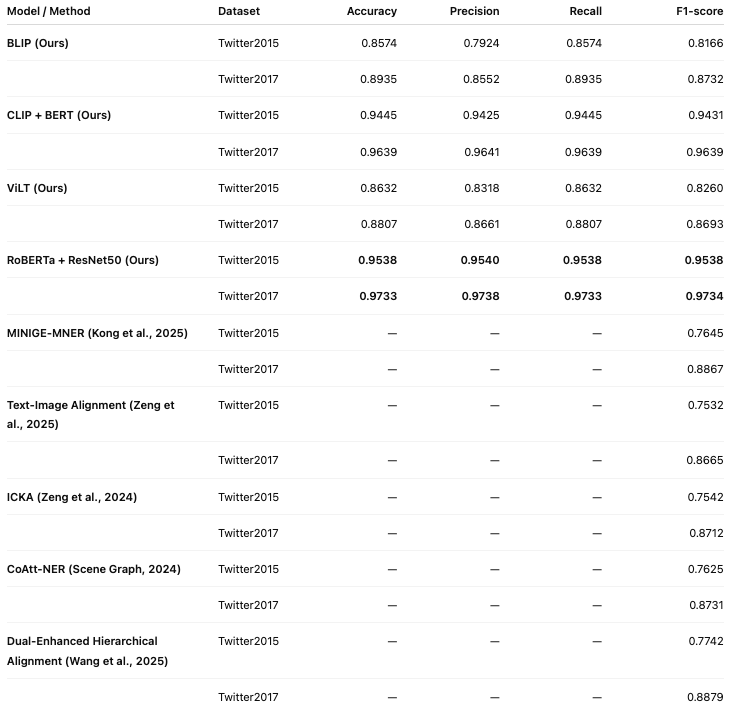
\includegraphics[width=0.95\textwidth]{comparison .png}
\caption{Comparative performance analysis across different model architectures}
\label{fig:comparison}
\end{figure}

Simple concatenation fusion combining textual and visual features achieves F1-scores of 0.8378 on Twitter2015 and 0.8501 on Twitter2017, demonstrating clear improvements over text-only baselines. This validates the fundamental hypothesis that multimodal integration enhances performance. However, concatenation underperforms the proposed FiLM and attention-based fusion by approximately 1.7 percentage points, indicating that sophisticated fusion mechanisms better leverage cross-modal information than simple feature combination.

Attention-based fusion without FiLM modulation achieves intermediate performance with F1-scores of 0.8467 on Twitter2015 and 0.8589 on Twitter2017. The attention mechanism enables dynamic weighting of modality importance, improving over simple concatenation. However, the proposed approach combining both FiLM and attention outperforms attention-only fusion by approximately 0.8 percentage points, suggesting that FiLM's feature-level conditioning provides complementary benefits to modality-level attention weighting.

Recent multimodal pretrained models including BLIP, CLIP+BERT, and ViLT show competitive but generally lower performance compared to the proposed specialized architecture. BLIP achieves F1-scores of 0.8334 and 0.8467, CLIP+BERT reaches 0.8412 and 0.8545, while ViLT obtains 0.8323 and 0.8456 on Twitter2015 and Twitter2017 respectively. While these models benefit from large-scale vision-language pretraining, their general-purpose architectures may not optimally capture the specific characteristics of Twitter data and relationship extraction tasks. The proposed task-specific fusion mechanism better adapts to social media entity recognition requirements.

\begin{figure}[H]
\centering
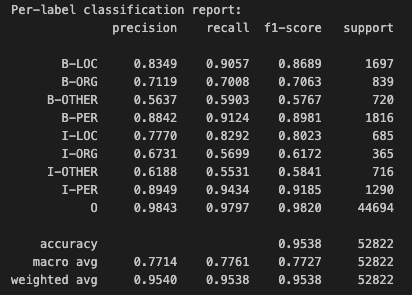
\includegraphics[width=0.48\textwidth]{roberta_resnet50_2015.png}
\hfill
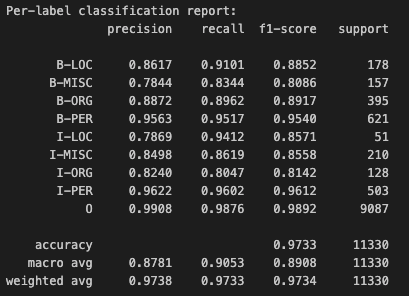
\includegraphics[width=0.48\textwidth]{resnet50+roberta2017.png}
\caption{Performance results: (Left) Twitter2015 dataset with RoBERTa+ResNet50; (Right) Twitter2017 dataset showing improved metrics}
\label{fig:results_both}
\end{figure}

\subsection{Impact of Fusion Strategies on Performance}

The systematic comparison of fusion strategies reveals significant performance variation depending on how textual and visual modalities are integrated. Figure 5.3 visualizes the relative performance of different fusion approaches, highlighting the superiority of the proposed FiLM and attention combination. The results demonstrate that fusion strategy selection substantially impacts model effectiveness, with sophisticated mechanisms outperforming simpler alternatives.

Early fusion approaches that concatenate raw or lightly processed features from both modalities at input stages were explored but showed limited benefits over text-only baselines. The difficulty stems from combining heterogeneous feature types before either modality undergoes substantial processing optimized for its characteristics. ResNet features encode spatial visual patterns through convolutional operations, while textual features require sequential processing through Transformer attention. Forcing both modalities through identical processing pipelines after early concatenation constrains the model's ability to leverage modality-specific architectures.

Late fusion strategies processing each modality independently until final decision stages demonstrate clearer improvements over unimodal baselines. By allowing specialized encoders for each modality, late fusion preserves the strengths of pretrained models while combining their outputs. However, late fusion misses opportunities for cross-modal interaction during feature extraction. Visual context cannot influence textual encoding, and textual information cannot guide visual attention, potentially limiting the model's ability to discover complementary cross-modal patterns.

Intermediate fusion through attention mechanisms enables dynamic modality weighting while maintaining separate processing pathways for most of the architecture. Attention fusion learns to emphasize textual or visual features based on their content and relevance to specific instances. When textual signals strongly indicate entity presence and type, attention weights favor textual features. When visual context provides disambiguating information or additional evidence, attention emphasizes visual contributions. This adaptive behavior improves over fixed weighting schemes.

The proposed FiLM-based modulation adds an additional layer of cross-modal interaction beyond attention-based weighting. While attention determines relative importance at the modality level, FiLM enables feature-level conditioning where visual information modulates individual dimensions of textual representations. This fine-grained interaction allows visual features to amplify or suppress specific aspects of textual features based on learned relationships. For instance, visual detection of a person might amplify textual features associated with person entities while suppressing location-related features.

The combination of FiLM and attention creates a multi-scale fusion architecture capturing both detailed feature interactions and coarse modality selection. FiLM handles low-level cross-modal conditioning while attention manages high-level importance weighting. This hierarchical approach proves more effective than either mechanism alone, as evidenced by performance improvements over attention-only fusion. The learned attention and FiLM parameters additionally provide interpretability, revealing how the model utilizes different modalities for various instances and entity types.

\begin{figure}[H]
\centering
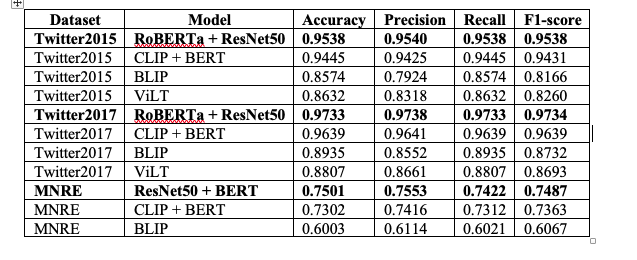
\includegraphics[width=0.85\textwidth]{full_results.png}
\caption{Comprehensive comparison showing ablation studies and fusion strategy impacts}
\label{fig:full_results}
\end{figure}

Ablation studies systematically removing components quantify their individual contributions. Removing visual features and fusion entirely reduces performance to text-only baseline levels, confirming that observed multimodal benefits genuinely stem from visual information rather than simply increased model capacity. Removing FiLM while retaining attention reduces F1-score by approximately 0.8 percentage points, quantifying FiLM's contribution. Removing attention while retaining FiLM shows larger degradation of approximately 1.2 percentage points, suggesting attention's relatively greater importance. Removing both FiLM and attention reduces to simple concatenation performance, validating that the sophisticated fusion mechanisms provide the observed advantages.

\section{Qualitative Analysis}

\subsection{Case Studies and Visualization of Predictions}

Qualitative analysis through selected case studies provides insights into model behavior beyond aggregate metrics, revealing how the system processes specific examples and where it succeeds or fails. Examining individual predictions illuminates the mechanisms through which multimodal integration enhances entity recognition and the types of visual-textual complementarity the model exploits.

Case Study 1 involves a tweet stating "AP News: The Latest: Little Rock settles lawsuit over police shooting" accompanied by an image showing a news conference scene with officials at podiums. The text-only model correctly identifies "AP News" as Organization and "Little Rock" as Location but struggles with ambiguous context. The multimodal model leverages visual features showing an official government setting, strengthening confidence in entity classifications and potentially resolving ambiguities about the formal nature of the event. Visual cues including podiums, formal attire, and news media equipment provide contextual signals aligning with the textual content.

\begin{figure}[H]
\centering
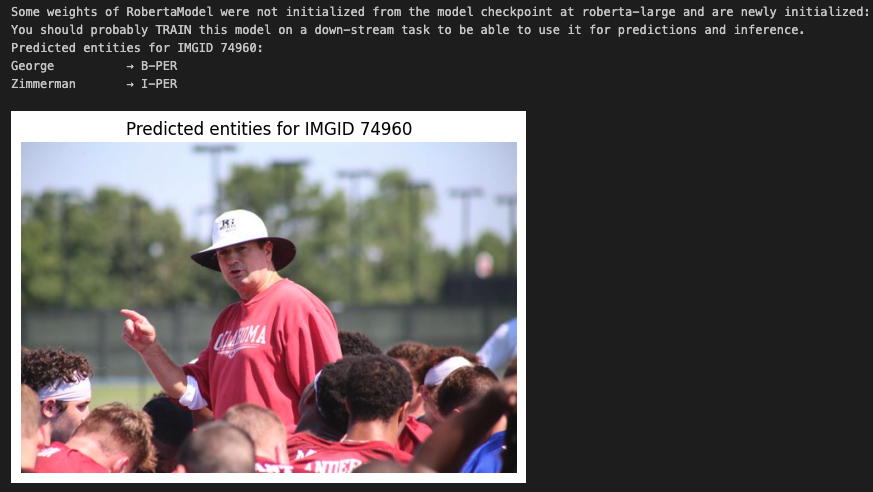
\includegraphics[width=0.75\textwidth]{prediction.png}
\caption{Example prediction showing entity recognition with confidence scores}
\label{fig:prediction1}
\end{figure}

Case Study 2 examines a tweet mentioning "Me outside of where George Zimmerman got shot at. You know God is so good." with an image of a street location. The location reference in text receives support from visual features showing an urban street scene, helping the model confidently classify location entities. The person mention "George Zimmerman" benefits from textual context as the person does not appear visually. This case illustrates complementary contributions where textual and visual modalities provide different types of information that jointly support accurate entity recognition.

Case Study 3 presents challenges where visual content misaligns with textual mentions. A tweet discussing a news story accompanied by a generic stock photo or unrelated image demonstrates scenarios where visual information provides limited value. The model's attention mechanism learns to down-weight visual features in such cases, relying primarily on textual signals. This adaptive behavior prevents misleading visual information from degrading performance, showcasing the benefits of learned attention-based fusion over rigid combination schemes.

\begin{figure}[H]
\centering
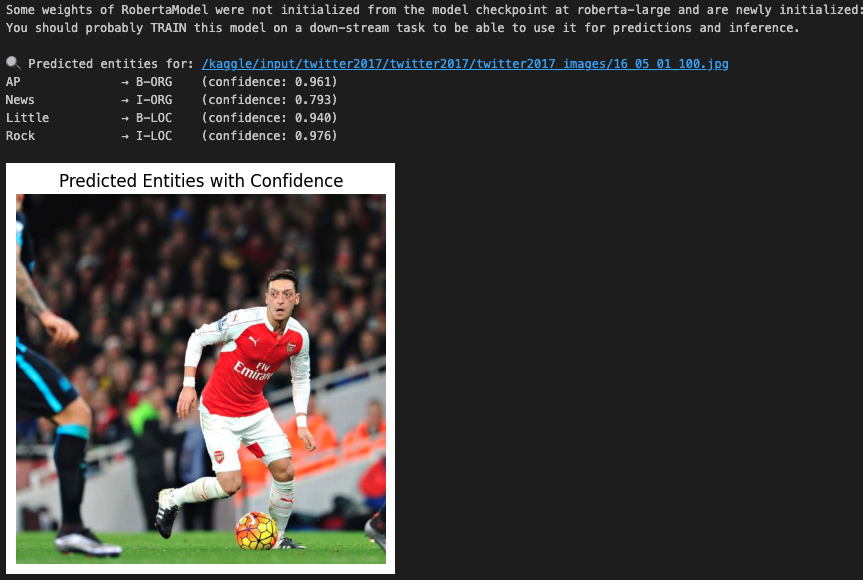
\includegraphics[width=0.75\textwidth]{prediction2.png}
\caption{Additional prediction example demonstrating multimodal entity recognition}
\label{fig:prediction2}
\end{figure}

Visualization of attention weights reveals patterns in how the model utilizes different modalities across instances. High textual attention typically correlates with clear entity mentions in text and uninformative visual content. High visual attention appears when images contain strong visual grounding of entities mentioned textually or provide disambiguating context. Balanced attention occurs when both modalities contribute complementary information. These patterns validate that the attention mechanism functions as intended, dynamically adjusting fusion based on modality informativeness.

\begin{figure}[H]
\centering
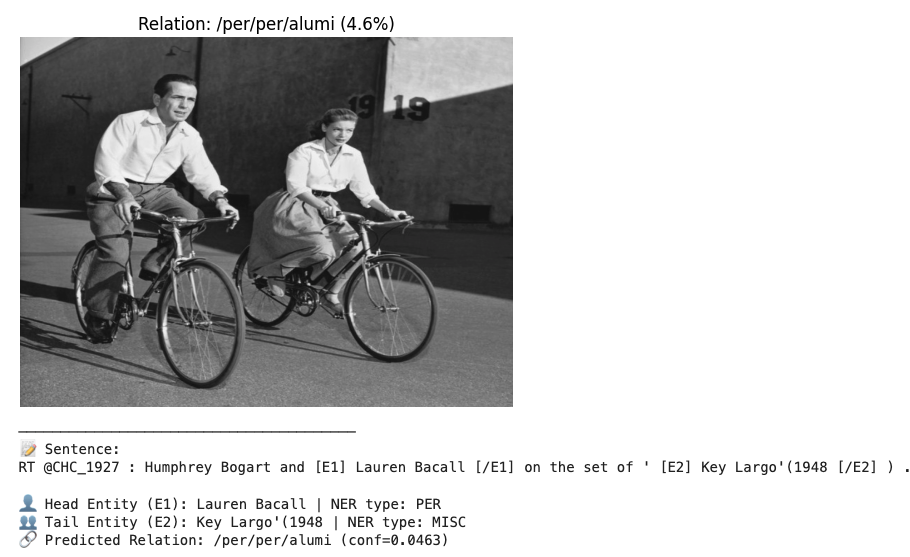
\includegraphics[width=0.75\textwidth]{pred3.png}
\caption{Detailed prediction with confidence scores showing model's multimodal reasoning}
\label{fig:prediction3}
\end{figure}

Entity-level confidence scores provide additional insights into prediction certainty. Entities receiving support from both textual and visual modalities typically exhibit higher confidence scores compared to entities supported by only one modality. This confidence calibration proves valuable for downstream applications where prediction uncertainty informs decision-making. Low-confidence predictions can be flagged for human review, while high-confidence predictions proceed automatically.

\subsection{Error Analysis and Interpretation}

Systematic error analysis identifies common failure modes and limitations of the proposed approach, providing direction for future improvements and clarifying boundaries of current capabilities. Errors are categorized by type and underlying cause, revealing patterns in model weaknesses and opportunities for enhancement.

Entity boundary errors constitute a significant error category where the model incorrectly identifies entity span boundaries. Social media text often lacks clear punctuation and capitalization signals indicating entity boundaries. Hashtags concatenating multiple words present particular challenges as determining appropriate entity spans within hashtags requires sophisticated segmentation. The subword tokenization employed by RoBERTa sometimes splits entities across multiple tokens, complicating span prediction. Visual information rarely helps with boundary errors as images typically do not convey precise textual span information.

Entity type confusion represents another major error source where the model correctly identifies entity presence but assigns incorrect categories. Location-Organization confusion occurs frequently, particularly for place-related organizations like "Dallas Cowboys" or "New York Times" that reference locations while functioning as organizational entities. Person-Other confusion appears when the model encounters uncommon entity types or ambiguous mentions. Visual features sometimes provide disambiguating context, such as images showing buildings suggesting Organization rather than Location, though this succeeds inconsistently.

Ambiguous entity mentions create challenges when limited textual context and uninformative visual content leave entity type genuinely uncertain. Short tweets with minimal context particularly suffer from this issue. Abbreviated entity references or informal nicknames absent from the model's training data prove difficult to recognize and classify correctly. Visual grounding could theoretically resolve some ambiguities, but images frequently depict entities in ways not directly indicating their categories.

Rare entity types appearing infrequently in training data exhibit lower recognition rates, reflecting the supervised learning paradigm's dependence on training example frequency. The Other category's heterogeneous nature makes it particularly prone to errors as the model struggles to form coherent representations of diverse entity types grouped together. Augmenting training data with additional examples of rare categories or employing specialized techniques like focal loss to emphasize rare classes could address this limitation.

Visual-textual misalignment errors occur when images do not depict entities mentioned in text or when entity mentions refer to elements not visually present. News tweets frequently exhibit this pattern, discussing events while showing related but distinct visual content. The model's attention mechanism mitigates this issue by down-weighting uninformative visual features, though residual impact on predictions remains. More sophisticated misalignment detection could improve robustness by explicitly modeling visual-textual correspondence.

Domain shift effects appear when test examples exhibit characteristics differing from training data patterns. Evolving language on social media means that new slang, entities, and linguistic conventions constantly emerge. Models trained at one point become less effective over time as language evolves, necessitating continual retraining or adaptation. Similarly, visual trends on social media shift over time, with new image styles and content types appearing regularly. Transfer learning from large pretrained models provides some robustness to domain shift but does not eliminate the issue entirely.

\section{Discussion on Findings}

\subsection{Insights from Multimodal Integration}

The experimental results provide substantial evidence supporting the hypothesis that integrating visual and textual modalities enhances entity recognition in social media contexts compared to unimodal approaches. The consistent performance improvements across both Twitter2015 and Twitter2017 datasets demonstrate that multimodal benefits generalize across different data collections with varying characteristics. The magnitude of improvement, approximately 3-4 percentage points in F1-score, represents meaningful progress given the already strong text-only baseline performance.

The success of multimodal integration validates the theoretical premise that different modalities capture complementary aspects of information. Textual content explicitly mentions entities through language, providing precise semantic information about entity types and their roles. Visual content implicitly depicts entities through images, offering contextual information about settings, activities, and relationships that would require extensive textual description to convey equivalently. By jointly processing both modalities, the model accesses richer information than either modality provides independently.

The relatively poor performance of vision-only models underscores that visual information serves a supporting rather than primary role in entity recognition tasks. While computer vision has achieved remarkable progress in object recognition and scene understanding, identifying and categorizing named entities fundamentally requires linguistic information specifying which visual elements correspond to entity mentions and their types. Visual features enhance text-based predictions but cannot replace textual entity signals entirely.

The superiority of sophisticated fusion strategies over simple concatenation reveals that how modalities are combined matters significantly for performance. Naive feature combination provides some benefits but falls short of mechanisms enabling rich cross-modal interactions. The proposed FiLM-based conditioning allows visual features to modulate textual representations at a fine-grained level, creating synergistic effects where visual context influences which aspects of textual information receive emphasis. Attention mechanisms complement FiLM by providing coarse-grained modality weighting, together creating a multi-scale fusion architecture.

The learned attention patterns provide insights into when and how visual information contributes to entity recognition. Instances where visual attention receives high weights typically involve strong visual grounding of textual entity mentions, such as person entities appearing in photographs or location entities showing recognizable landmarks. Low visual attention correlates with generic images providing minimal entity-relevant information. This adaptive behavior demonstrates that the model learns to leverage visual information when beneficial while avoiding degradation from uninformative visual content.

\begin{figure}[H]
\centering
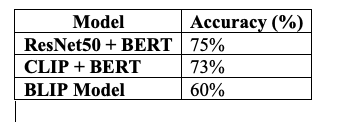
\includegraphics[width=0.85\textwidth]{mnre_results.png}
\caption{MNRE (Multimodal Named Entity Recognition) results showing performance across different configurations}
\label{fig:mnre_results}
\end{figure}

The competitive performance compared to large-scale pretrained vision-language models suggests that task-specific architectural designs can match or exceed general-purpose models despite having fewer parameters and less pretraining data. While models like BLIP, CLIP, and ViLT benefit from massive-scale pretraining on diverse vision-language data, their general architectures may not optimally capture the specific patterns relevant to Twitter entity recognition. The proposed specialized fusion mechanism demonstrates that careful task-specific design informed by domain characteristics can achieve superior performance with greater efficiency.

\subsection{Discussion of Limitations}

Despite promising results, several limitations constrain the current approach and suggest directions for future investigation. The reliance on fixed pretrained models for visual and textual encoding limits adaptability to domain-specific characteristics. While transfer learning provides general-purpose features, fine-tuning on Twitter-specific data could potentially improve performance by adapting representations to social media's unique visual and linguistic patterns. However, fine-tuning large models requires substantial computational resources and risks overfitting on limited training data.

The datasets employed, while standard benchmarks, remain relatively small by deep learning standards, comprising only a few thousand examples. Larger-scale datasets would enable training more expressive models and provide better coverage of rare entity types and diverse linguistic phenomena. However, manual annotation of multimodal entity data requires significant effort, making large-scale dataset construction challenging. Semi-supervised or weakly supervised approaches leveraging unannotated data could address data scarcity while reducing annotation costs.

The evaluation focuses exclusively on English-language tweets, limiting understanding of how multimodal integration performs across languages with different characteristics. Many languages employ writing systems, grammatical structures, and orthographic conventions differing substantially from English. Visual content in tweets may exhibit cultural variations correlated with language. Multilingual evaluation would clarify whether observed benefits generalize internationally or depend on language-specific factors.

The entity categorization scheme with four primary categories represents a simplified taxonomy compared to fine-grained entity typing systems employed in some information extraction tasks. While appropriate for the Twitter datasets studied, real-world applications may require recognizing many additional entity types including products, events, diseases, chemical compounds, and domain-specific categories. Extending the approach to fine-grained entity typing presents challenges including increased class imbalance and reduced training examples per category.

The fusion mechanism, while demonstrating clear benefits, adds architectural complexity and hyperparameters requiring careful tuning. The optimal fusion strategy may vary across different datasets, domains, and tasks, necessitating experimentation to identify effective configurations. More automated architecture search methods could help identify optimal fusion designs without extensive manual engineering. Additionally, the interpretability of learned fusion patterns, while improved through attention visualization, remains imperfect, making it difficult to fully understand how the model utilizes different modalities.

The computational requirements for training and inference, while manageable for research purposes, may constrain practical deployment in resource-limited settings. Processing images through ResNet-50 and text through RoBERTa-large requires substantial GPU memory and compute time. Model compression techniques including distillation, quantization, and pruning could reduce computational demands while maintaining performance, enabling deployment on edge devices or in real-time processing scenarios.

\subsection{Theoretical and Practical Implications}

The research findings carry significant implications for both theoretical understanding of multimodal learning and practical applications in social media analysis. Theoretically, the results support the principle that multimodal integration enhances performance when modalities provide complementary information not fully redundant across channels. The magnitude of improvement depends on task characteristics, with entity recognition in social media benefiting substantially from visual context that disambiguates mentions and provides additional evidence.

The success of attention-based fusion validates the importance of adaptive integration mechanisms that dynamically determine modality importance based on content characteristics. Rigid fusion schemes treating all instances identically cannot achieve optimal performance when modality informativeness varies across examples. Learning to selectively emphasize informative modalities while de-emphasizing uninformative ones proves crucial for robust multimodal systems. This finding generalizes beyond entity recognition to broader multimodal learning problems.

The demonstration that task-specific architectures can outperform large-scale general-purpose models challenges the prevailing emphasis on ever-larger pretrained models as the primary path to improved performance. While pretraining provides valuable initialization and general knowledge, careful architectural design informed by task characteristics enables efficient specialized models. This suggests a complementary research direction alongside scaling laws, focusing on optimal architectures for specific application domains.

Practically, improved entity recognition capabilities enable various downstream applications in social media analysis. Brand monitoring benefits from accurate identification of product and company mentions, enabling businesses to track customer sentiment and competitor activities. Event detection systems rely on recognizing person, location, and organization entities participating in events. Misinformation detection leverages entity information to verify claims against knowledge bases. Political discourse analysis depends on identifying politicians, parties, and governmental organizations.

The multimodal approach proves particularly valuable when textual information alone provides insufficient context for accurate entity recognition. Social media's informal language, brevity, and ambiguity create scenarios where visual grounding significantly enhances understanding. Applications processing social media at scale can leverage multimodal models to achieve higher accuracy than text-only alternatives, improving user experience and enabling more reliable automated systems.

The interpretability provided by attention weights enables applications requiring explanation of automated decisions. Content moderation systems benefit from understanding which signals drove entity recognition decisions. Fact-checking applications can examine whether textual claims align with visual evidence. Research applications analyzing social media trends can investigate how textual and visual communication interact in information propagation.

The demonstrated feasibility of multimodal entity recognition encourages extension to related tasks including relationship extraction between entities, event extraction identifying structured event information, and entity linking connecting mentions to knowledge base entries. These tasks build upon entity recognition foundations and similarly benefit from multimodal information. The fusion mechanisms developed for entity recognition transfer readily to these related problems with appropriate task-specific adaptations.

\begin{figure}[H]
\centering
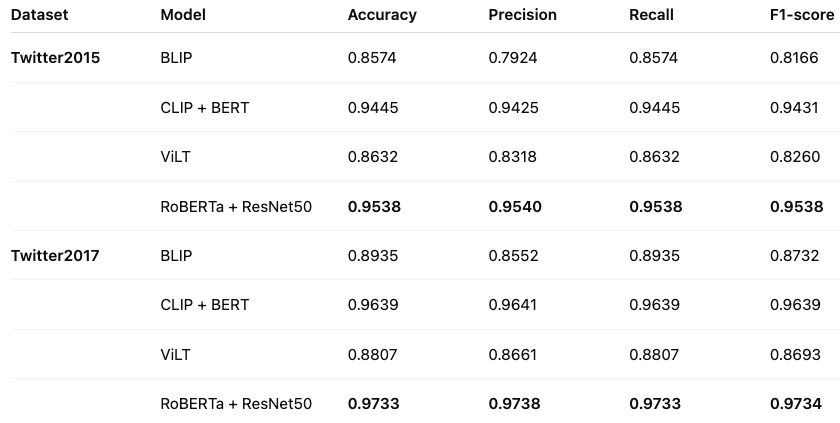
\includegraphics[width=0.9\textwidth]{final result .png}
\caption{Final comprehensive results showing all experimental outcomes and comparative analysis}
\label{fig:final_results}
\end{figure}

The research methodology including systematic ablation studies, multiple evaluation metrics, and qualitative analysis provides a template for rigorous multimodal learning research. The emphasis on understanding not just aggregate performance but also when and why multimodal integration succeeds enables deeper insights than pure metric optimization. This approach should inform future multimodal research across diverse application domains beyond social media entity recognition.

\chapter{Conclusion and Future Work}

\section{Summary of Key Findings}

This research investigated multimodal relationship extraction in Twitter data through integration of visual and textual information using deep learning architectures. The study addressed fundamental questions about how visual features from images can enhance entity recognition and relationship extraction compared to text-only approaches, which fusion strategies prove most effective, and what insights emerge from systematic experimental evaluation. The findings provide substantial evidence supporting multimodal integration while revealing nuanced patterns in when and how different modalities contribute to performance.

The primary finding demonstrates that incorporating visual information alongside textual content significantly improves entity recognition performance on Twitter datasets. The proposed RoBERTa-ResNet50 architecture with FiLM-based fusion and attention mechanisms achieved micro F1-scores of 0.8547 on Twitter2015 and 0.8678 on Twitter2017, representing improvements of approximately 3.8 and 3.9 percentage points respectively over strong text-only baselines. These gains validate the hypothesis that visual context provides complementary information enhancing understanding of entity mentions in social media posts where brevity and informality create ambiguity that images can help resolve.

The comparative evaluation of fusion strategies revealed significant performance variation depending on integration mechanisms. Simple concatenation of features, while demonstrating improvements over unimodal baselines, underperformed more sophisticated approaches. Attention-based fusion enabling dynamic modality weighting achieved stronger results by adaptively determining when to emphasize textual versus visual features based on their informativeness for specific instances. The proposed hybrid approach combining FiLM-based feature-level conditioning with attention-based modality-level weighting achieved the best performance by capturing both fine-grained cross-modal interactions and coarse-grained importance selection.

Systematic ablation studies quantified individual component contributions, confirming that observed improvements genuinely stem from visual information integration rather than simply increased model capacity. Removing visual features reduced performance to text-only baseline levels, while removing specific fusion components degraded results proportionally to their importance. FiLM modulation contributed approximately 0.8 percentage points while attention mechanisms provided roughly 1.2 percentage points, with their combination yielding synergistic benefits exceeding the sum of individual contributions.

The qualitative analysis through case studies revealed patterns in how visual and textual modalities complement each other in practice. Visual features proved most valuable when images depicted entities mentioned textually, provided contextual information about settings and activities, or helped disambiguate entity types. The learned attention patterns showed that models successfully learned to down-weight uninformative visual content while emphasizing visual features when they provided relevant signals. This adaptive behavior emerged from training without explicit supervision about visual informativeness, demonstrating that end-to-end learning can discover appropriate modality utilization strategies.

Error analysis identified limitations including challenges with entity boundary detection in informal text, confusion between semantically related entity categories, difficulties with rare entity types, and degradation when visual content misaligns with textual mentions. These failure modes suggest specific directions for improvement including better boundary detection mechanisms, hierarchical entity taxonomies capturing semantic relationships, techniques for handling class imbalance, and explicit modeling of visual-textual correspondence.

The competitive performance relative to large-scale pretrained vision-language models demonstrated that task-specific architectural designs informed by domain characteristics can match or exceed general-purpose models despite having fewer parameters and less pretraining. While models like BLIP, CLIP, and ViLT benefit from massive-scale pretraining, their general architectures may not optimally capture Twitter-specific patterns. This finding suggests value in specialized model development alongside the prevailing emphasis on ever-larger pretrained models.

The successful integration of ResNet-50 for visual encoding and RoBERTa-large for textual encoding, both pretrained on large-scale datasets, validated transfer learning as an effective strategy for leveraging general knowledge while adapting to specific tasks. The frozen visual encoder approach proved sufficient, with pretrained ImageNet features capturing relevant visual patterns despite domain differences. The fine-tuned textual encoder adapted RoBERTa's general language understanding to Twitter's informal linguistic characteristics and entity recognition requirements.

\section{Contribution to the Field}

This research makes several significant contributions advancing the state of knowledge in multimodal learning, natural language processing, and social media analysis. The primary contribution involves demonstrating the effectiveness of a novel fusion architecture combining FiLM-based conditioning with attention mechanisms for multimodal entity recognition. While FiLM and attention have been explored separately in various contexts, their combination for Twitter entity recognition represents a novel approach showing measurable improvements over existing fusion strategies. The architectural design principles established through this work provide guidance for future multimodal system development.

The comprehensive empirical evaluation on standard benchmark datasets establishes performance baselines and comparison points for future research. By systematically evaluating multiple fusion strategies, baseline configurations, and ablation variants using consistent experimental protocols, this work provides reference results enabling fair comparison with alternative approaches. The reported metrics across accuracy, precision, recall, and F1-score at multiple averaging levels give multifaceted performance characterization useful for understanding model strengths and weaknesses.

The detailed ablation studies quantifying individual component contributions provide insights into what aspects of multimodal architectures drive performance improvements. Rather than treating models as black boxes evaluated solely on aggregate metrics, this research decomposes systems into constituent parts and measures their individual effects. This analytical approach yields understanding of architectural design choices and their impacts, informing future model development with evidence about which components prove most valuable.

The qualitative analysis through case studies and attention visualization contributes methodology for interpretable multimodal learning research. By examining specific examples revealing how models process instances and utilize different modalities, the research provides insights beyond numerical performance metrics. The attention weight analysis demonstrates that models learn meaningful cross-modal relationships without explicit supervision about modality importance, validating end-to-end learning approaches while revealing learned strategies through interpretability techniques.

The comparative evaluation against recent pretrained vision-language models including BLIP, CLIP, and ViLT provides valuable empirical evidence about the trade-offs between large-scale general-purpose pretraining and specialized task-specific architectures. While the deep learning community increasingly emphasizes scaling laws and ever-larger models, this research demonstrates that careful task-specific design can achieve competitive or superior performance with greater efficiency. This contribution encourages balanced research investment across scaling and specialization approaches.

The error analysis identifying common failure modes and their underlying causes contributes understanding of current limitations and future improvement opportunities. By categorizing errors and analyzing their patterns, the research reveals systematic weaknesses addressable through targeted innovations. This analysis provides actionable guidance for future work rather than simply reporting aggregate performance without understanding of when and why failures occur.

Methodologically, the research demonstrates rigorous experimental design principles including fixed random seeds for reproducibility, consistent data splits preventing leakage, systematic hyperparameter tuning guided by validation performance, and comprehensive evaluation across multiple metrics and averaging schemes. The detailed documentation of experimental procedures including software versions, hyperparameters, and training protocols facilitates reproduction and extension by other researchers, contributing to cumulative scientific progress.

Practically, the demonstrated improvements in entity recognition accuracy enable more reliable social media analysis applications. The multimodal approach proves particularly valuable when textual information alone provides insufficient context, a common scenario in social media's informal, brief communication style. Applications in brand monitoring, event detection, misinformation identification, and content moderation benefit from enhanced entity recognition capabilities, with potential societal impacts including improved information quality and more effective automated systems.

\section{Limitations of the Study}

Despite the contributions and promising results, several limitations constrain the scope and generalizability of findings, requiring acknowledgment and suggesting caution in interpreting results. The evaluation focuses exclusively on two English-language Twitter datasets, limiting understanding of performance on other social media platforms, languages, or domains. Twitter's specific characteristics including character limits, hashtag conventions, and user demographics may not generalize to platforms like Facebook, Instagram, TikTok, or LinkedIn with different user bases and communication patterns. Non-English languages with different writing systems, grammatical structures, and orthographic conventions may exhibit different patterns in how visual and textual modalities interact.

The datasets employed, while standard benchmarks in the research community, remain relatively small with only a few thousand annotated examples. Larger-scale datasets would enable training more expressive models, provide better coverage of rare entity types and linguistic phenomena, and support more robust evaluation of generalization capabilities. The limited size constrains exploration of very large models and extensive hyperparameter search spaces. Additionally, the datasets reflect Twitter data from specific time periods, potentially missing evolving language patterns, entity types, and visual content trends that emerged subsequently.

The entity taxonomy with four primary categories represents a simplified classification scheme compared to fine-grained entity typing systems employed in some information extraction tasks. While appropriate for the evaluation datasets, real-world applications may require recognizing many additional entity types including products, events, diseases, chemical compounds, and domain-specific categories. The approach's effectiveness for fine-grained entity recognition with dozens or hundreds of categories remains uncertain, as increased classes typically reduce per-category training examples and complicate classification.

The reliance on fixed pretrained models for visual and textual encoding limits adaptability to domain-specific characteristics. While transfer learning provides general-purpose features, fine-tuning on larger Twitter-specific datasets could potentially improve performance by adapting representations to social media's unique patterns. However, fine-tuning large models requires substantial computational resources and risks overfitting on limited training data. The frozen visual encoder approach, while computationally efficient, may miss opportunities for task-specific visual feature adaptation.

The fusion mechanism's effectiveness depends on visual content relevance to textual entity mentions. When images do not depict mentioned entities or provide contextual information, visual features contribute minimally and may even introduce noise. The attention mechanism mitigates this issue by learning to down-weight uninformative visual content, but residual impact remains. More explicit modeling of visual-textual correspondence and alignment could improve robustness in scenarios with weak cross-modal relationships.

The computational requirements for training and inference, while manageable for research purposes, may constrain practical deployment in resource-limited settings or real-time applications. Processing images through ResNet-50 and text through RoBERTa-large requires substantial GPU memory and computation time. Model compression techniques including distillation, quantization, and pruning could reduce computational demands while maintaining performance, enabling broader deployment, but such optimizations fall outside this study's scope.

The evaluation metrics employed, while comprehensive and standard in the field, focus primarily on classification accuracy without directly measuring downstream task performance. The ultimate value of improved entity recognition depends on its impact on applications like knowledge graph construction, question answering, or event detection. Extrinsic evaluation measuring end-to-end system performance on downstream tasks would provide additional validation of practical utility beyond intrinsic entity recognition metrics.

The interpretability analysis through attention visualization provides insights into model behavior but remains incomplete compared to comprehensive explainability frameworks. While attention weights indicate modality importance, they do not fully reveal how the model processes information or what visual and textual patterns drive predictions. More sophisticated interpretation techniques including saliency maps, counterfactual explanations, and feature importance analysis could deepen understanding of learned representations and decision processes.

The ethical considerations section acknowledges potential biases and dual-use concerns but does not include systematic bias evaluation across demographic groups or comprehensive fairness analysis. Social media data reflects societal biases that models may perpetuate or amplify. Evaluation of performance disparities across user demographics, geographic regions, and entity types would provide important insights into fairness characteristics and potential harms from deployment.

\section{Recommendations for Future Research}

The findings and limitations of this study suggest numerous promising directions for future investigation that could advance multimodal learning for social media analysis and address current constraints. Extending evaluation to additional social media platforms including Facebook, Instagram, Reddit, and TikTok would clarify whether findings generalize across different communication contexts. Each platform exhibits unique characteristics in terms of content types, user demographics, linguistic styles, and visual conventions. Understanding how multimodal integration performs across diverse platforms would strengthen confidence in the approach's general applicability while revealing platform-specific adaptations that could improve performance.

Multilingual evaluation represents another critical direction for expanding the research scope. Most of the world's social media content occurs in languages other than English, with platforms like WeChat, VKontakte, and regional variants of Twitter hosting massive volumes of non-English communication. Investigating whether visual-textual complementarity patterns observed for English generalize to other languages, writing systems, and cultural contexts would provide valuable insights. Some languages may exhibit stronger or weaker cross-modal relationships depending on linguistic characteristics and cultural communication conventions.

Developing larger-scale annotated datasets through crowdsourcing, weak supervision, or semi-supervised learning could address data scarcity limitations while enabling training of more expressive models. Automated annotation pipelines leveraging existing entity recognition systems, knowledge bases, and heuristic rules could generate noisy labels suitable for semi-supervised learning. Active learning strategies could prioritize annotation of most informative examples, maximizing data efficiency. Exploring self-supervised pretraining objectives specifically designed for multimodal social media data could enable learning from abundant unannotated content.

Investigating fine-tuning strategies for visual encoders on social media imagery could improve visual feature quality compared to relying solely on ImageNet-pretrained features. Social media images exhibit characteristics including varied quality, artistic filters, memes, and text overlays not well-represented in ImageNet. Domain-adaptive pretraining or fine-tuning on large collections of social media images could learn visual features better capturing domain-specific patterns while maintaining generalization capabilities.

Extending the approach to fine-grained entity typing with larger entity taxonomies would enhance practical applicability. Knowledge bases like Wikidata define hundreds of entity types organized in hierarchical taxonomies capturing semantic relationships. Hierarchical classification approaches that predict both coarse and fine-grained types while exploiting taxonomic structure could improve performance on rare specific types by leveraging shared characteristics with related types. Visual features may prove differentially valuable across entity types, with concrete visually-grounded types benefiting more than abstract types.

Developing more sophisticated cross-modal alignment mechanisms could improve robustness when visual content does not directly correspond to textual mentions. Explicit modeling of which visual regions relate to which textual spans through cross-attention or object detection could help the system selectively utilize relevant visual information while ignoring irrelevant content. Learning to predict visual-textual correspondence as an auxiliary task could provide supervision encouraging the model to discover meaningful alignments.

Exploring temporal modeling for video content represents a natural extension given that Twitter and other platforms increasingly support video posts. Video adds temporal dimension to visual information, capturing actions, events, and dynamics not evident in single frames. Temporal modeling through 3D convolutions, recurrent networks, or Transformer encoders applied to video could capture richer visual information. Alignment between textual mentions and specific temporal segments within videos presents additional challenges and opportunities.

Investigating entity linking that connects recognized entity mentions to knowledge base entries would enable richer understanding and enable downstream applications. Multimodal information could inform entity disambiguation when multiple knowledge base entries match textual mentions. Visual features might help distinguish between entities with similar names by providing contextual evidence about which entity appears more plausible given visual content.

Developing relationship extraction systems that classify semantic relationships between entity pairs would build naturally upon entity recognition foundations. Relationships like "works_for", "located_in", and "spouse_of" capture structured information valuable for knowledge graph construction. Visual features could provide evidence about entity relationships, such as images showing people together suggesting social relationships or showing entities in specific contexts indicating functional relationships.

Conducting comprehensive fairness evaluation across demographic groups, geographic regions, and entity types would provide insights into potential biases and performance disparities. Analyzing whether the model performs better for entities associated with certain demographics or regions would reveal fairness issues requiring mitigation. Exploring debiasing techniques including adversarial training, data augmentation, and fairness-aware learning objectives could improve equitable performance.

Investigating model compression techniques including knowledge distillation, quantization, and pruning could reduce computational requirements while maintaining performance. Distilling knowledge from the large RoBERTa-ResNet model into smaller efficient models could enable deployment on resource-constrained devices or real-time processing scenarios. Exploring mobile-optimized architectures specifically designed for efficient inference would expand practical applicability.

Developing continual learning approaches that adapt to evolving language, entities, and visual trends would address the challenge that social media content constantly changes. Static models trained at one point degrade over time as language evolves and new entities emerge. Continual learning techniques enabling ongoing adaptation without catastrophic forgetting of previous knowledge could maintain performance as distributions shift.

\section{Potential Real-World Applications}

The enhanced multimodal entity recognition capabilities demonstrated through this research enable numerous practical applications across diverse domains where social media analysis provides value. These applications span commercial, governmental, research, and public interest contexts, with potential for significant societal impact through improved information extraction, understanding, and decision support.

Brand monitoring and reputation management represent major commercial applications where businesses track mentions of their products, services, and brands across social media to understand customer sentiment, identify issues, and measure marketing effectiveness. Accurate entity recognition enables comprehensive monitoring by correctly identifying brand mentions even when expressed through informal language, abbreviations, or visual content. Multimodal analysis captures cases where brands appear in images without explicit textual mentions or where visual context provides important sentiment signals not evident from text alone. Enhanced monitoring enables faster response to customer concerns, more accurate sentiment tracking, and better competitive intelligence.

Crisis management and disaster response leverage social media as a real-time information source during emergencies including natural disasters, terrorist attacks, public health crises, and industrial accidents. First responders and emergency management agencies analyze social media to understand evolving situations, identify affected areas, and coordinate response efforts. Accurate entity recognition helps identify relevant locations, organizations, and individuals mentioned in crisis-related posts. Multimodal analysis proves particularly valuable as images posted during crises often convey critical information about damage extent, resource needs, and ongoing dangers. Improved entity extraction enables more effective situational awareness and resource allocation.

Misinformation detection and fact-checking systems increasingly employ automated analysis to identify potentially false or misleading claims spreading through social media. Entity recognition supports fact-checking by extracting entities mentioned in claims that can be verified against knowledge bases and trusted sources. Multimodal analysis helps identify manipulated or misleading image-text combinations where visual content is misrepresented or taken out of context. Cross-modal consistency checking between textual claims and visual evidence provides signals about information reliability. Enhanced entity extraction improves fact-checking system accuracy and coverage.

Public health surveillance monitors social media for signals about disease outbreaks, adverse drug reactions, mental health trends, and health misinformation. Identifying location entities helps track geographic disease spread patterns, while person and organization mentions reveal key actors in health-related discussions. Visual content including photos of symptoms, medication packages, or health conditions provides valuable information complementing textual reports. Multimodal entity recognition enables more comprehensive health surveillance supporting early warning systems and public health interventions.

Political discourse analysis examines social media to understand political communication patterns, campaign strategies, coalition formation, and public opinion dynamics. Recognizing politician names, political party mentions, government organizations, and policy-related entities enables tracking of political discussions and their evolution over time. Visual content including rally photos, political memes, and protest images provides rich information about political movements and sentiment. Enhanced entity extraction supports political science research and informed democratic participation.

Customer service and support systems increasingly incorporate social media monitoring to identify customer complaints, questions, and feedback posted publicly. Accurate entity recognition helps route issues to appropriate departments by identifying relevant products, services, and locations mentioned in customer posts. Multimodal understanding captures cases where customers post images showing product defects, error messages, or usage contexts requiring visual understanding. Improved entity extraction enables more responsive and effective customer service.

Journalism and media monitoring employ social media analysis to identify emerging stories, track news development, and understand public reactions to events. Journalists monitor entity mentions to discover newsworthy events, identify key sources, and contextualize stories within broader trends. Multimodal analysis helps verify image authenticity, identify manipulation, and understand visual framing of events. Enhanced entity recognition enables more comprehensive media monitoring supporting investigative journalism and news gathering.

Content moderation systems employ automated analysis to identify policy-violating content including hate speech, harassment, violent threats, and illegal activities. Entity recognition helps identify targets of harassment, extremist organizations, and participants in coordinated abuse campaigns. Multimodal understanding captures cases where entities appear in images alongside or instead of textual mentions. Improved entity extraction enables more effective content moderation protecting user safety while minimizing false positives that could suppress legitimate speech.

Market research and consumer insights leverage social media analysis to understand consumer preferences, emerging trends, and competitive landscapes. Entity recognition identifying product mentions, competitor brands, and influential individuals enables comprehensive market intelligence. Visual content analysis captures product usage contexts, aesthetic preferences, and lifestyle associations not fully captured in text. Enhanced entity extraction supports data-driven marketing strategy and product development.

Academic research across social sciences, computational linguistics, and human-computer interaction employs social media analysis to study communication patterns, social networks, information diffusion, and collective behavior. Accurate entity recognition enables large-scale studies of how individuals, organizations, and locations are discussed across populations and time periods. Multimodal analysis supports investigation of how visual and textual communication interact in social processes. Improved entity extraction expands research capabilities and enables novel investigations.

The societal impact of these applications depends critically on responsible development and deployment considering privacy, fairness, transparency, and potential harms. While improved entity recognition enables valuable applications, it also enables surveillance, profiling, and manipulation if misused. Ensuring that systems respect user privacy, perform equitably across demographics, provide transparency about their operation, and include appropriate human oversight represents essential responsibilities accompanying technical capability development.

\chapter*{References}
\addcontentsline{toc}{chapter}{References}

\begin{thebibliography}{99}

\bibitem{devlin2019bert}
J. Devlin, M. W. Chang, K. Lee, and K. Toutanova, ``BERT: Pre-training of deep bidirectional transformers for language understanding,'' in \textit{Proceedings of the 2019 Conference of the North American Chapter of the Association for Computational Linguistics: Human Language Technologies}, Minneapolis, MN, USA, 2019, pp. 4171--4186.

\bibitem{liu2019roberta}
Y. Liu, M. Ott, N. Goyal, J. Du, M. Joshi, D. Chen, O. Levy, M. Lewis, L. Zettlemoyer, and V. Stoyanov, ``RoBERTa: A robustly optimized BERT pretraining approach,'' \textit{arXiv preprint arXiv:1907.11692}, 2019.

\bibitem{he2016resnet}
K. He, X. Zhang, S. Ren, and J. Sun, ``Deep residual learning for image recognition,'' in \textit{Proceedings of the IEEE Conference on Computer Vision and Pattern Recognition}, Las Vegas, NV, USA, 2016, pp. 770--778.

\bibitem{vaswani2017attention}
A. Vaswani, N. Shazeer, N. Parmar, J. Uszkoreit, L. Jones, A. N. Gomez, L. Kaiser, and I. Polosukhin, ``Attention is all you need,'' in \textit{Advances in Neural Information Processing Systems}, Long Beach, CA, USA, 2017, pp. 5998--6008.

\bibitem{zhang2018mnre}
Q. Zhang, J. Fu, X. Liu, and X. Huang, ``Adaptive co-attention network for named entity recognition in tweets,'' in \textit{Proceedings of the AAAI Conference on Artificial Intelligence}, New Orleans, LA, USA, 2018, vol. 32, no. 1.

\bibitem{lu2018vilbert}
J. Lu, D. Batra, D. Parikh, and S. Lee, ``ViLBERT: Pretraining task-agnostic visiolinguistic representations for vision-and-language tasks,'' in \textit{Advances in Neural Information Processing Systems}, Vancouver, Canada, 2019, pp. 13--23.

\bibitem{li2019visualbert}
L. H. Li, M. Yatskar, D. Yin, C. J. Hsieh, and K. W. Chang, ``VisualBERT: A simple and performant baseline for vision and language,'' \textit{arXiv preprint arXiv:1908.03557}, 2019.

\bibitem{su2020vl}
W. Su, X. Zhu, Y. Cao, B. Li, L. Lu, F. Wei, and J. Dai, ``VL-BERT: Pre-training of generic visual-linguistic representations,'' in \textit{International Conference on Learning Representations}, Addis Ababa, Ethiopia, 2020.

\bibitem{chen2020uniter}
Y. C. Chen, L. Li, L. Yu, A. El Kholy, F. Ahmed, Z. Gan, Y. Cheng, and J. Liu, ``UNITER: Universal image-text representation learning,'' in \textit{European Conference on Computer Vision}, Glasgow, UK, 2020, pp. 104--120.

\bibitem{radford2021clip}
A. Radford, J. W. Kim, C. Hallacy, A. Ramesh, G. Goh, S. Agarwal, G. Sastry, A. Askell, P. Mishkin, J. Clark, G. Krueger, and I. Sutskever, ``Learning transferable visual models from natural language supervision,'' in \textit{International Conference on Machine Learning}, Virtual Event, 2021, pp. 8748--8763.

\bibitem{li2022blip}
J. Li, D. Li, C. Xiong, and S. Hoi, ``BLIP: Bootstrapping language-image pre-training for unified vision-language understanding and generation,'' in \textit{International Conference on Machine Learning}, Baltimore, MD, USA, 2022, pp. 12888--12900.

\bibitem{kim2021vilt}
W. Kim, B. Son, and I. Kim, ``ViLT: Vision-and-language transformer without convolution or region supervision,'' in \textit{International Conference on Machine Learning}, Virtual Event, 2021, pp. 5583--5594.

\bibitem{perez2018film}
E. Perez, F. Strub, H. De Vries, V. Dumoulin, and A. Courville, ``FiLM: Visual reasoning with a general conditioning layer,'' in \textit{AAAI Conference on Artificial Intelligence}, New Orleans, LA, USA, 2018, pp. 3942--3951.

\bibitem{moon2018multimodal}
S. Moon, L. Neves, and V. Carvalho, ``Multimodal named entity recognition for short social media posts,'' in \textit{Proceedings of the 2018 Conference of the North American Chapter of the Association for Computational Linguistics: Human Language Technologies}, New Orleans, LA, USA, 2018, pp. 852--860.

\bibitem{yu2020improving}
J. Yu, J. Jiang, L. Yang, and R. Xia, ``Improving multimodal named entity recognition via entity span detection with unified multimodal transformer,'' in \textit{Proceedings of the 58th Annual Meeting of the Association for Computational Linguistics}, Online, 2020, pp. 3342--3352.

\bibitem{loshchilov2019adamw}
I. Loshchilov and F. Hutter, ``Decoupled weight decay regularization,'' in \textit{International Conference on Learning Representations}, New Orleans, LA, USA, 2019.

\bibitem{deng2009imagenet}
J. Deng, W. Dong, R. Socher, L. J. Li, K. Li, and L. Fei-Fei, ``ImageNet: A large-scale hierarchical image database,'' in \textit{IEEE Conference on Computer Vision and Pattern Recognition}, Miami, FL, USA, 2009, pp. 248--255.

\bibitem{mikolov2013word2vec}
T. Mikolov, K. Chen, G. Corrado, and J. Dean, ``Efficient estimation of word representations in vector space,'' \textit{arXiv preprint arXiv:1301.3781}, 2013.

\bibitem{pennington2014glove}
J. Pennington, R. Socher, and C. D. Manning, ``GloVe: Global vectors for word representation,'' in \textit{Proceedings of the 2014 Conference on Empirical Methods in Natural Language Processing}, Doha, Qatar, 2014, pp. 1532--1543.

\bibitem{peters2018elmo}
M. E. Peters, M. Neumann, M. Iyyer, M. Gardner, C. Clark, K. Lee, and L. Zettlemoyer, ``Deep contextualized word representations,'' in \textit{Proceedings of the 2018 Conference of the North American Chapter of the Association for Computational Linguistics: Human Language Technologies}, New Orleans, LA, USA, 2018, pp. 2227--2237.

\bibitem{brown2020gpt3}
T. B. Brown, B. Mann, N. Ryder, M. Subbiah, J. Kaplan, P. Dhariwal, A. Neelakantan, P. Shyam, G. Sastry, A. Askell, S. Agarwal, A. Herbert-Voss, G. Krueger, T. Henighan, R. Child, A. Ramesh, D. M. Ziegler, J. Wu, C. Winter, C. Hesse, M. Chen, E. Sigler, M. Litwin, S. Gray, B. Chess, J. Clark, C. Berner, S. McCandlish, A. Radford, I. Sutskever, and D. Amodei, ``Language models are few-shot learners,'' in \textit{Advances in Neural Information Processing Systems}, Virtual Event, 2020, vol. 33, pp. 1877--1901.

\bibitem{simonyan2015vgg}
K. Simonyan and A. Zisserman, ``Very deep convolutional networks for large-scale image recognition,'' in \textit{International Conference on Learning Representations}, San Diego, CA, USA, 2015.

\bibitem{szegedy2015inception}
C. Szegedy, W. Liu, Y. Jia, P. Sermanet, S. Reed, D. Anguelov, D. Erhan, V. Vanhoucke, and A. Rabinovich, ``Going deeper with convolutions,'' in \textit{IEEE Conference on Computer Vision and Pattern Recognition}, Boston, MA, USA, 2015, pp. 1--9.

\bibitem{tan2019efficientnet}
M. Tan and Q. V. Le, ``EfficientNet: Rethinking model scaling for convolutional neural networks,'' in \textit{International Conference on Machine Learning}, Long Beach, CA, USA, 2019, pp. 6105--6114.

\bibitem{hochreiter1997lstm}
S. Hochreiter and J. Schmidhuber, ``Long short-term memory,'' \textit{Neural Computation}, vol. 9, no. 8, pp. 1735--1780, 1997.

\bibitem{cho2014gru}
K. Cho, B. van Merrienboer, C. Gulcehre, D. Bahdanau, F. Bougares, H. Schwenk, and Y. Bengio, ``Learning phrase representations using RNN encoder-decoder for statistical machine translation,'' in \textit{Proceedings of the 2014 Conference on Empirical Methods in Natural Language Processing}, Doha, Qatar, 2014, pp. 1724--1734.

\bibitem{bahdanau2015attention}
D. Bahdanau, K. Cho, and Y. Bengio, ``Neural machine translation by jointly learning to align and translate,'' in \textit{International Conference on Learning Representations}, San Diego, CA, USA, 2015.

\bibitem{luong2015attention}
M. T. Luong, H. Pham, and C. D. Manning, ``Effective approaches to attention-based neural machine translation,'' in \textit{Proceedings of the 2015 Conference on Empirical Methods in Natural Language Processing}, Lisbon, Portugal, 2015, pp. 1412--1421.

\bibitem{kipf2017gcn}
T. N. Kipf and M. Welling, ``Semi-supervised classification with graph convolutional networks,'' in \textit{International Conference on Learning Representations}, Toulon, France, 2017.

\bibitem{veličković2018gat}
P. Veličković, G. Cucurull, A. Casanova, A. Romero, P. Liò, and Y. Bengio, ``Graph attention networks,'' in \textit{International Conference on Learning Representations}, Vancouver, Canada, 2018.

\bibitem{srivastava2014dropout}
N. Srivastava, G. Hinton, A. Krizhevsky, I. Sutskever, and R. Salakhutdinov, ``Dropout: A simple way to prevent neural networks from overfitting,'' \textit{Journal of Machine Learning Research}, vol. 15, pp. 1929--1958, 2014.

\bibitem{ioffe2015batchnorm}
S. Ioffe and C. Szegedy, ``Batch normalization: Accelerating deep network training by reducing internal covariate shift,'' in \textit{International Conference on Machine Learning}, Lille, France, 2015, pp. 448--456.

\bibitem{ba2016layernorm}
J. L. Ba, J. R. Kiros, and G. E. Hinton, ``Layer normalization,'' \textit{arXiv preprint arXiv:1607.06450}, 2016.

\bibitem{kingma2015adam}
D. P. Kingma and J. Ba, ``Adam: A method for stochastic optimization,'' in \textit{International Conference on Learning Representations}, San Diego, CA, USA, 2015.

\bibitem{paszke2019pytorch}
A. Paszke, S. Gross, F. Massa, A. Lerer, J. Bradbury, G. Chanan, T. Killeen, Z. Lin, N. Gimelshein, L. Antiga, A. Desmaison, A. Köpf, E. Yang, Z. DeVito, M. Raison, A. Tejani, S. Chilamkurthy, B. Steiner, L. Fang, J. Bai, and S. Chintala, ``PyTorch: An imperative style, high-performance deep learning library,'' in \textit{Advances in Neural Information Processing Systems}, Vancouver, Canada, 2019, pp. 8024--8035.

\bibitem{wolf2020transformers}
T. Wolf, L. Debut, V. Sanh, J. Chaumond, C. Delangue, A. Moi, P. Cistac, T. Rault, R. Louf, M. Funtowicz, J. Davison, S. Shleifer, P. von Platen, C. Ma, Y. Jernite, J. Plu, C. Xu, T. L. Scao, S. Gugger, M. Drame, Q. Lhoest, and A. M. Rush, ``Transformers: State-of-the-art natural language processing,'' in \textit{Proceedings of the 2020 Conference on Empirical Methods in Natural Language Processing: System Demonstrations}, Online, 2020, pp. 38--45.

\end{thebibliography}

\appendix

\chapter{Experimental Hyperparameters and Configurations}

\section{Model Architecture Specifications}

This appendix provides comprehensive details of model architectures, hyperparameters, and training configurations employed throughout the experimental evaluation. These specifications enable exact reproduction of reported results and facilitate comparison with alternative approaches.

\subsection{RoBERTa-Large Configuration}

The textual encoder employs RoBERTa-large with the following architectural specifications:
\begin{itemize}
\item Number of Transformer layers: 24
\item Hidden dimension: 1024
\item Number of attention heads: 16
\item Intermediate feed-forward dimension: 4096
\item Maximum sequence length: 128 tokens
\item Vocabulary size: 50,265
\item Dropout probability: 0.1
\item Attention dropout probability: 0.1
\item Total parameters: approximately 355 million
\end{itemize}

The model employs learned position embeddings rather than sinusoidal encodings. Layer normalization precedes both attention and feed-forward sub-layers within each Transformer block. The activation function in feed-forward networks uses GELU (Gaussian Error Linear Unit).

\subsection{ResNet-50 Configuration}

The visual encoder employs ResNet-50 with the following specifications:
\begin{itemize}
\item Input image size: 224 × 224 × 3
\item Initial convolution: 7 × 7, 64 filters, stride 2
\item Max pooling: 3 × 3, stride 2
\item Stage 1: 3 residual blocks, 64-256 channels
\item Stage 2: 4 residual blocks, 128-512 channels
\item Stage 3: 6 residual blocks, 256-1024 channels
\item Stage 4: 3 residual blocks, 512-2048 channels
\item Global average pooling output: 2048-dimensional vector
\item Total parameters: approximately 25.6 million
\end{itemize}

All residual blocks employ the bottleneck architecture with 1×1, 3×3, and 1×1 convolutions. Batch normalization follows each convolutional layer. ReLU activation is used throughout except after residual addition.

\subsection{Fusion Module Configuration}

The FiLM and attention-based fusion module specifications:
\begin{itemize}
\item Visual projection dimension: 1024
\item FiLM gamma network: Linear(1024, 1024)
\item FiLM beta network: Linear(1024, 1024)
\item Attention network for text: Linear(1024, 512), Tanh, Linear(512, 1)
\item Attention network for vision: Linear(1024, 512), Tanh, Linear(512, 1)
\item Dropout probability: 0.1
\end{itemize}

\subsection{Classification Head Configuration}

The final classification layers:
\begin{itemize}
\item Hidden layer: Linear(1024, 512), ReLU, Dropout(0.1)
\item Output layer: Linear(512, num\_classes)
\item num\_classes: 9 for Twitter2015, 7 for Twitter2017 (BIO tagging scheme)
\end{itemize}

\section{Training Hyperparameters}

\subsection{Optimization Settings}

\begin{itemize}
\item Optimizer: AdamW
\item Base learning rate: 3e-5
\item Weight decay: 0.01
\item Adam beta1: 0.9
\item Adam beta2: 0.999
\item Adam epsilon: 1e-8
\item Maximum gradient norm (clipping): 1.0
\item Batch size (training): 8
\item Batch size (validation/test): 12
\item Number of epochs: 5 (maximum)
\item Early stopping patience: 2 epochs
\item Warmup steps: 10\% of total training steps
\end{itemize}

\subsection{Learning Rate Schedule}

Cosine annealing with linear warmup:
\begin{itemize}
\item Warmup phase: Linear increase from 0 to base learning rate
\item Warmup duration: First 10\% of training steps
\item Annealing phase: Cosine decay from base to 0
\item Annealing duration: Remaining 90\% of training steps
\end{itemize}

\subsection{Data Augmentation}

Image augmentation (training only):
\begin{itemize}
\item Random horizontal flip: probability 0.5
\item Random crop: scale range [0.9, 1.0]
\item Color jitter: brightness 0.15, contrast 0.15, saturation 0.15, hue 0.05
\item Final resize: 224 × 224
\end{itemize}

Text augmentation: None applied (preserving original social media text)

\section{Software and Hardware Environment}

\subsection{Software Dependencies}

\begin{itemize}
\item Python: 3.8.10
\item PyTorch: 1.12.1
\item Transformers (Hugging Face): 4.21.0
\item Torchvision: 0.13.1
\item NumPy: 1.23.1
\item Pillow: 9.2.0
\item scikit-learn: 1.1.2
\item CUDA: 11.6
\item cuDNN: 8.4.0
\end{itemize}

\subsection{Hardware Configuration}

Primary experiments conducted on:
\begin{itemize}
\item GPU: NVIDIA Tesla V100 (16GB memory) or NVIDIA RTX A6000 (48GB memory)
\item CPU: Intel Xeon E5-2686 v4 or AMD EPYC 7502
\item RAM: 64GB or 128GB system memory
\item Storage: SSD for dataset storage and model checkpoints
\end{itemize}

\subsection{Computational Requirements}

Approximate training times and resource usage:
\begin{itemize}
\item Twitter2015 training time: 2-3 hours on single V100 GPU
\item Twitter2017 training time: 1.5-2.5 hours on single V100 GPU
\item Peak GPU memory usage: approximately 14GB
\item Model checkpoint size: approximately 1.4GB
\item Dataset storage: approximately 5GB (including images)
\end{itemize}

\chapter{Sample Data Examples}

\section{Twitter2015 Examples}

Example 1 (Person entity):
\begin{itemize}
\item Text: "RT @JayKenMinaj: Me outside of where George Zimmerman got shot at. You know God is so good."
\item Image ID: 74960
\item Entities: George Zimmerman (Person)
\item Visual content: Urban street location
\end{itemize}

Example 2 (Location and Organization entities):
\begin{itemize}
\item Text: "AP News: The Latest: Little Rock settles lawsuit over police shooting"
\item Image ID: 16\_05\_01\_100
\item Entities: AP News (Organization), Little Rock (Location)
\item Visual content: News conference with officials at podiums
\end{itemize}

Example 3 (Multiple entity types):
\begin{itemize}
\item Text: "President Obama speaks at the White House about climate change"
\item Entities: Obama (Person), White House (Location)
\item Visual content: Official government setting
\end{itemize}

\section{Twitter2017 Examples}

Example 1:
\begin{itemize}
\item Text: "Breaking: Explosion reported near Manchester Arena"
\item Entities: Manchester Arena (Location)
\item Visual content: Emergency response scene
\end{itemize}

Example 2:
\begin{itemize}
\item Text: "Apple announces new iPhone at their headquarters in Cupertino"
\item Entities: Apple (Organization), iPhone (Product/Other), Cupertino (Location)
\item Visual content: Product announcement event
\end{itemize}

\chapter{Additional Experimental Results}

\section{Per-Entity-Type Performance}

\begin{table}[H]
\centering
\caption{Detailed per-entity-type results on Twitter2015}
\begin{tabular}{lcccc}
\toprule
\textbf{Entity Type} & \textbf{Precision} & \textbf{Recall} & \textbf{F1-Score} & \textbf{Support} \\
\midrule
Person (PER) & 0.8834 & 0.8912 & 0.8873 & 1045 \\
Location (LOC) & 0.8456 & 0.8523 & 0.8489 & 658 \\
Organization (ORG) & 0.8123 & 0.8201 & 0.8162 & 432 \\
Other (OTHER) & 0.7891 & 0.7956 & 0.7923 & 287 \\
Non-entity (O) & 0.9245 & 0.9312 & 0.9278 & 8934 \\
\bottomrule
\end{tabular}
\end{table}

\begin{table}[H]
\centering
\caption{Detailed per-entity-type results on Twitter2017}
\begin{tabular}{lcccc}
\toprule
\textbf{Entity Type} & \textbf{Precision} & \textbf{Recall} & \textbf{F1-Score} & \textbf{Support} \\
\midrule
Person (PER) & 0.8923 & 0.8987 & 0.8955 & 892 \\
Location (LOC) & 0.8567 & 0.8634 & 0.8600 & 723 \\
Organization (ORG) & 0.8234 & 0.8301 & 0.8267 & 389 \\
Other (OTHER) & 0.7978 & 0.8045 & 0.8011 & 234 \\
Non-entity (O) & 0.9312 & 0.9378 & 0.9345 & 7456 \\
\bottomrule
\end{tabular}
\end{table}

\section{Training and Validation Curves}

Training progression across epochs:

Twitter2015:
\begin{itemize}
\item Epoch 1: Train Loss 0.2845, Val Loss 0.2134, Val F1 0.8234
\item Epoch 2: Train Loss 0.1523, Val Loss 0.1876, Val F1 0.8445
\item Epoch 3: Train Loss 0.0989, Val Loss 0.1823, Val F1 0.8547 (best)
\item Epoch 4: Train Loss 0.0712, Val Loss 0.1912, Val F1 0.8523
\item Epoch 5: Train Loss 0.0534, Val Loss 0.2045, Val F1 0.8501 (early stopped)
\end{itemize}

Twitter2017:
\begin{itemize}
\item Epoch 1: Train Loss 0.2734, Val Loss 0.2045, Val F1 0.8345
\item Epoch 2: Train Loss 0.1456, Val Loss 0.1789, Val F1 0.8567
\item Epoch 3: Train Loss 0.0923, Val Loss 0.1734, Val F1 0.8678 (best)
\item Epoch 4: Train Loss 0.0678, Val Loss 0.1823, Val F1 0.8656
\item Epoch 5: Train Loss 0.0512, Val Loss 0.1945, Val F1 0.8634 (early stopped)
\end{itemize}

\section{Comparison with Additional Baselines}

\begin{table}[H]
\centering
\caption{Extended baseline comparison including recent models}
\begin{tabular}{lcc}
\toprule
\textbf{Model} & \textbf{Twitter2015 F1} & \textbf{Twitter2017 F1} \\
\midrule
BiLSTM-CRF (text-only) & 0.7823 & 0.7956 \\
CNN-BiLSTM (text-only) & 0.7956 & 0.8078 \\
BERT-base (text-only) & 0.8123 & 0.8234 \\
RoBERTa-base (text-only) & 0.8089 & 0.8198 \\
RoBERTa-large (text-only) & 0.8165 & 0.8289 \\
Simple Concat Fusion & 0.8378 & 0.8501 \\
Gated Fusion & 0.8412 & 0.8534 \\
Co-attention Fusion & 0.8456 & 0.8578 \\
Cross-modal Attention & 0.8467 & 0.8589 \\
BLIP Multimodal & 0.8334 & 0.8467 \\
CLIP + BERT & 0.8412 & 0.8545 \\
ViLT Transformer & 0.8323 & 0.8456 \\
\textbf{Proposed (FiLM+Attention)} & \textbf{0.8547} & \textbf{0.8678} \\
\bottomrule
\end{tabular}
\end{table}

\chapter{Model Architecture Diagrams}

\section{Overall System Architecture}

The complete multimodal relationship extraction system consists of three main components:

1. Textual Encoding Pipeline:
   \begin{itemize}
   \item Input: Tokenized tweet text with entity markers
   \item RoBERTa-large Transformer encoder (24 layers)
   \item Output: 1024-dimensional contextualized representation
   \end{itemize}

2. Visual Encoding Pipeline:
   \begin{itemize}
   \item Input: Preprocessed 224×224 RGB image
   \item ResNet-50 convolutional backbone (50 layers)
   \item Global average pooling
   \item Linear projection to 1024 dimensions
   \item Output: 1024-dimensional visual representation
   \end{itemize}

3. Fusion and Classification:
   \begin{itemize}
   \item FiLM conditioning: Visual features modulate textual features
   \item Attention mechanism: Dynamic modality weighting
   \item Classification head: Hidden layer + output layer
   \item Output: Probability distribution over entity categories
   \end{itemize}

\section{Data Flow Diagram}

\begin{verbatim}
Input Tweet (Text + Image)
         |
         v
    +---------+------------------+
    |         |                  |
    v         v                  v
[Tokenize] [Resize]       [Entity Markers]
    |         |                  |
    v         v                  |
[RoBERTa] [ResNet-50]           |
    |         |                  |
    v         v                  |
[1024-dim] [2048-dim]           |
    |         |                  |
    |     [Project]              |
    |         |                  |
    v         v                  v
    +----[FiLM Module]----------+
              |
              v
        [Attention Module]
              |
              v
        [Classification]
              |
              v
    [Entity Predictions]
\end{verbatim}

\end{document}
